\documentclass{article} % For LaTeX2e
\usepackage{iclr2017_conference,times}
\usepackage{hyperref}
\usepackage{url}
% \usepackage[dvips]{graphicx}

% from Exploring Policy Rep
\usepackage[utf8]{inputenc}
\usepackage{hyperref}
\usepackage{amssymb}
\usepackage{amsmath}
\usepackage[normalem]{ulem}
\usepackage{dsfont}

\usepackage{subfigure}
\newcommand{\R}{\mathbb{R}}
\renewcommand{\S}{\mathcal{S}}
\newcommand{\A}{\mathcal{A}}
\newcommand{\EE}{\mathbb{E}}
\usepackage{changepage}
\usepackage{graphicx}

\usepackage{pdfpages}

\usepackage{cancel}

\title{Stochastic Neural Networks for \\Hierarchical Reinforcement Learning}


\author{Carlos Florensa${^\dagger}$, Yan Duan${^\dagger}{^\ddagger}$, Pieter Abbeel${^\dagger}{^\ddagger}$ \\
$^\dagger$ UC Berkeley, Department of Electrical Engineering and Computer Science\\
$^\ddagger$ OpenAI\\
% Department of Electrical Engineering and Computer Sciences\\
% UC Berkeley\\
\texttt{florensa@berkeley.edu, \{rocky,pieter\}@openai.edu}
}

% The \author macro works with any number of authors. There are two commands
% used to separate the names and addresses of multiple authors: \And and \AND.
%
% Using \And between authors leaves it to \LaTeX{} to determine where to break
% the lines. Using \AND forces a linebreak at that point. So, if \LaTeX{}
% puts 3 of 4 authors names on the first line, and the last on the second
% line, try using \AND instead of \And before the third author name.

\newcommand{\fix}{\marginpar{FIX}}
\newcommand{\new}{\marginpar{NEW}}

%\iclrfinalcopy % Uncomment for camera-ready version

\begin{document}
	
	\maketitle

\begin{abstract}


Deep reinforcement learning has achieved many impressive results in recent years. However, many of the deep RL algorithms still employ naive exploration strategies, and they have been shown to perform poorly in tasks with sparse rewards, and/or with a long horizon. To tackle these challenges, there are two common approaches. The first approach is to design a hierarchy over the actions, which would require domain-specific knowledge and careful hand-engineering. A different line of work utilizes domain-agnostic intrinsic rewards to guide exploration, which has been shown to be effective in tasks with sparse rewards. However, it is unclear how the knowledge of solving a task can be utilized for other tasks, leading to a high sample complexity overall. In this paper, we propose a general framework for learning useful skills in a pre-training environment, which can then be utilized in downstream tasks by training a high-level policy over these skills. To learn these skills, we use stochastic neural networks (SNNs) combine with an intrinsic reward, the design of which requires very minimal domain knowledge about the downstream tasks. Our experiments show that this combination is effective in learning a wide span of interpretable skills in a sample-efficient way, and, when trained on downstream tasks, can significantly boost the learning performance uniformly across all tasks.

% Many practical problems in Reinforcement Learning (RL) only have a high level reward signal. This includes all tasks where a reward is only received when reaching a certain goal, even if many coordinated actions need to be taken before. Therefore these tasks have a \textit{sparse reward} and are considered some of the hardest in the field. To tackle them the two main approaches are reward shaping (eg. with some intrinsic motivation for exploration bonus) or using hand-engineered sequences of actions that allow to hierarchize the task and take high level actions (\textit{skills}, \textit{macro-actions} or \textit{options}). The first method can be completely unsupervised but the learning for one specific goal is difficult to re-use for another goal, even if the underlying dynamics are the same. The second method grants better re-use of skills but the prior knowledge needed to design the \textit{macro-actions} is undesired. In the present work we combine the best of both worlds to obtain \textit{skills} in a completely unsupervised fashion via a pre-training step and then use them to solve the actual task. We prove that a good "span of skills" can be learned using Stochastic Neural Networks (SNN) given their extra expressive power. The property of yielding different solutions to the MDP at the end of training (instead of a single one as most RL algorithms) is very interesting and we outline other uses in domain adaptation and bad local minima avoidance.
\end{abstract}

\section{Introduction}

% - What is the problem?
% - Why is it interesting and important?
% - Why is it hard? (E.g., why do naive approaches fail?) OK
% - Why hasn't it been solved before? (Or, what's wrong with previous proposed solutions? How does mine differ?)
% - What are the key components of my approach and results? Also include any specific limitations.


In recent years, deep reinforcement learning has achieved many impressive results, including playing Atari games using raw pixel inputs \citep{NIPS2014_5421, Mnih15, Schulman15TRPO}, mastering the game of Go \citep{ silver2016mastering}, and acquiring advanced manipulation and locomotion skills from raw sensory inputs \citep{Schulman15TRPO, lillicrap2015continuous, watter2015embed, schulman2016high, heess2015learning, levine2016end}.
% These successes can be traced back to much earlier work \citep{Tesauro95TDGammon, Bertsekas95Neuro}.
Despite these success stories, these deep RL algorithms typically employ naive exploration strategies such as $\epsilon$-Greedy or uniform Gaussian exploration noise, which have been shown to perform poorly in tasks with sparse rewards \citep{duan2016benchmarking, houthooft2016variational, bellemare2016unifying}.
Tasks with sparse rewards are common in realistic scenarios. 
For example, in navigation tasks, the agent is not rewarded until it finds the target. The challenge is further complicated by long horizons, where naive exploration strategies can lead to exponentially large sample complexity \citep{osband2014generalization}.

To tackle these challenges, there are two natural strategies.
The first strategy is to design a hierarchy over the actions \citep{parr1998reinforcement, sutton1999between, dietterich2000hierarchical}.
%%TODO: more recent citations here?
By composing low-level actions into high-level primitives, the search space can be reduced exponentially, leading to much faster learning. However, although these approaches can be effective, they require domain-specific knowledge and careful hand-engineering. Another line of work uses intrinsic rewards to guide exploration \citep{schmidhuber1991curious, schmidhuber2010formal, houthooft2016variational, bellemare2016unifying}.
The computation of these intrinsic rewards does not require domain-specific knowledge, and the same approach can be applied to a wide range of tasks.
However, when facing a collection of tasks, these methods do not provide a direct answer about how knowledge about solving one task may transfer to other tasks, and by solving each of the tasks from scratch, the overall sample complexity may still be high.%the overall sample complexity may still be high.
% Rocky: I'm not too satisfied with this argument..

In this paper, we propose a general framework for training policies in a collection of tasks with sparse rewards.
Our framework first learns a span of skills in a pre-training environment, where it is employed with nothing but an intrinsic reward signal, whose design only require very minimal domain knowledge about the downstream tasks.
The set of skills can be used later in a wide collection of different tasks, by training a separate high-level policy for each task on top of the skills, thus reducing sample complexity uniformly.
To learn the span of skills, we propose to use stochastic neural networks (SNNs) \citep{neal1990learning, neal1992connectionist, tang2013learning}, a class of neural networks with stochastic units in the computation graph.
This class of architecture can easily represent multi-modal policies, while achieving weight sharing among the different modes.
We parametrize the stochasticity in the network by feeding latent variables with simple distributions as extra input to the policy.
By varying the latent code input, and executing the policy conditioned on the latent code, we obtain different behaviors of the policy.
However, direct application of stochastic neural networks does not always guarantee that a wide range of skills will be learned. 
We propose an information-theoretic regularizer in the pre-training phase to encourage diversity of behaviors of the SNN policy.
Our experiments find that our hierarchical policy-learning framework can learn a wide range of skills, which are clearly interpretable as the latent code is varied. Furthermore, we show that training high-level policies on top of the learned skills can lead to great performance on a set of challenging tasks with long horizon and sparse rewards. %The span of skills learned during the pre-training phase are clearly interpretable, outperforming methods in comparison that do not use SNN policies, or .

%Combined together, we show that % stochastic neural network %, to be learnt, and we show that . %has greater expressive power than usual feed-forward neural networks 

%We show that the % about these downstream tasks, while 


% Recent advances in Deep Reinforcement Learning allow to train agents with super-human performance in tasks with discrete action-space like Go \cite{2016go} or some Atari games \cite{mnih2015human}. Nevertheless, many challenges remain in the continuous state-action environments, and in particular the problem of tasks with sparse reward is even more acute in the continuous case. In robotics, tasks like navigation or manipulation only have a natural reward in the goal position, and it is often hard to provide constant supervision along the trajectories with a cost function tailored to the task [cite IRL litterature?]. The main difficulty is that a sequence of well coordinated actions, producing a purposeful motion, is required to get any reward signal. Hence, as has been reported in the recent benchmark for continuous control tasks \cite{yuan2015}, it is very unlikely that the usual $\epsilon$-Greedy or Boltzmann exploration [ref] or adding Gaussian noise to the controls for policy gradient algorithms [TRPO], will yield a trajectory providing any feedback. 

% To tackle this issue/challenge there are two main approaches and in this paper we will combine the best of both. One consists in providing an exploration bonus to the agent so that, despite not getting to the goal, it is still pushed to explore unseen regions that could potentially contain the extrinsic reward. In discrete MDPs this intrinsic reward may take many forms, from the simplest based on state-counting (rewarding each state inversely proportional to a function of its visitation counts) [refm, DM, simHash] to information theory-based like surprisal [ ref!! ]. In the continuous domain, VIME uses variatinal inference in Bayesian neural networks to incentivize exploration.

% it is common to provide a specific abstraction of the problem.

% Furthermore, interested in performing well in new environments without much experience in it. This is concretized in the following problem statement.

% Words from ICLR call for papers:
% - Unsupervised
% - Representation learning for planning and reinforcement learning
% - Hierarchical models
% - application to robotics


\section{Related Work}

% Nothing!

% jk

One of the main appeals of hierarchical reinforcement learning (HRL) is to use skills to reduce the search complexity of the problem \citep{parr1998reinforcement, sutton1999between, dietterich2000hierarchical}. The concept of skills has been formalized by the options framework proposed by \cite{sutton1999between}. Automatic learning of skills is a central question in HRL to avoid heavy hand-engineering of the hierarchical structure, and there has been a lot of work on discovering options [cite a bunch]. However, very few work has been done on Also review
deepmind's paper%one of the central questions in hierarchical reinforcement leanring [cite a bunch], a central queLearning a Hierarchical reinforcement learning 


Our use of stochastic neural networks is inspired by a large body of previous work.
There is a large body of work on stochastic neural networks.  restricted boltzmann machines, deep belief networks, sigmoid belief networks. Recently they have been applied to generative modeling of complicated distributions [cite VAE, GAN].

Our setup of a collection of downstream tasks belongs to the general category of multi-task reinforcement learning. cite a bunch

Intrinsic rewards have been used in reinforcement learning as an auxiliary training signal in addition to the true rewards.

Our information-theoretic regularizer is based on encouraging mutual information between the latent variables and the visitation frequency in the state space. This is inspired by the recent success of using information regularization to enforce interpretability of the latent codes in generative adversarial nets (GANs) \citep{chen2016infogan}.

%been more commonly known as generative models.
%Stochastic neural networks have been studied in the past

% - Previous stochastic neural networks literature
% - Literature on HRL
% - Very importantly, deepmind's recent work, and how our work is situated compared to theirs
% - Multi-task learning literature
% - Intrinsic rewards. How they are used; what 
% - Mutual information regularizer. Cite InfoGAN




\section{Preliminaries}
\subsection{MDP}
\begin{itemize}
    \item This paper assumes a finite-horizon discounted Markov decision process (MDP), defined by $(\S,\A,P, R, \rho_0, \gamma, T)$, in which $\S$ is the state space, $\A$ the action space, $P$ a transition probability distribution, $R$ a reward function, $\rho_0$ an initial state distribution,  $\gamma \in (0, 1]$ a discount factor, and $T$ the horizon. The goal of RL is to maximize the total expected discounted reward $\EE_{\pi} \left[\sum_{t=0}^T \gamma^t R(s_t, a_t) \right]$ over policy $\pi$, which outputs a distribution over actions given a state.
    %describe MDP?
    \item introduce "intrinsic rewards" (COM speed)
\end{itemize}

\subsection{Stochastic Neural Networks}

\begin{itemize}
    \item To solve continuous MDPS with Policy Gradient methods \citep{peters2008reinforcement}, a stochastic policy is required [appart if you do DDPG?]. The usual is to use a deterministic neural network to parametrize the mean $\mu(s_t)$ and variance $\Sigma(s_t)$ of a Gaussian distribution, from where the next action $a_{t+1}$ is sampled. From the re-parametrization trick perspective \citep{look at SVG paper or DeepMind-modulate}, this corresponds to simply having a linear combination of normal noise at the output of the neural network:
    \begin{equation}
        a_{t+1} = \mu_{\theta}(s_t) +\epsilon \Sigma_\theta(s_t), ~~~~ \epsilon \sim \mathbb{N}(0,I)
    \end{equation}
    \item Hence, despite the arbitrary expresiveness of the neural networks, the noise addition process is very restricted, with two major drawbacks. On one hand the exploration is limited and this process will not perform well for continuous sparse hierarchical tasks. 
    
    On the other hand the policy will be unimodal by construction!
\end{itemize}
The usual Stochastic Feedforward Neural Networks were first described by \citet{tang2013sfnn}

\subsection{Bilinear Integration of latents}

\section{Problem statement}
In robotics we are usually interested in solving a collection of tasks with common underlying dynamics. For example, in navigation it is not enough to learn how to solve a single maze: we want to be able to solve other mazes with the same robot. Furthermore it is desirable to leverage off-line experience to reduce the training time needed from each specific task. 

More formally we consider the problem of minimizing the average samples needed to solve a collection of MDPs $\{m_i\}_{i\in I}$ drawn from a certain distribution:
\begin{equation}
    m_i = (\mathcal{S}_i, \mathcal{A}_i, \mathcal{P}_i, r_i, \rho_{0i}, \gamma_i, T_i) \sim \mathbb{P}_{MDP}\big( (\cdot, \cdot, \cdot, \cdot, \cdot, \cdot, \cdot) \big)
\end{equation}
\textit{[This is not too good notation: I should impose that for any element in P, not for the particular samples I had]}
This distribution has the particularity of having a common \textit{inner structure} $(\mathcal{S}_{in}, \mathcal{A}_{in}, \mathcal{P}_{in})$ satisfying \textit{[is this too restrictive? should I generalize more?]}
$$\mathcal{S}_{in} \subset \mathcal{S}_i,~~ \mathcal{A}_{in} = \mathcal{A}_i,~~ \mathcal{P}_i(s)=f(\mathcal{P}_{in}(s))~~~ \forall i\in I$$
This can correspond to the dynamics of the robot or to some other invariant part of the MDPs to which we have access offline. The challenge is to leverage the partial information provided by the triplet $(\mathcal{S}_{in}, \mathcal{A}_{in}, \mathcal{P}_{in})$ in a pre-train phase so that the performance in $\{m_i\}_{i\in I}$ is improved.

\section{Methodology}

Despite having access to $(\mathcal{S}_{in}, \mathcal{A}_{in}, \mathcal{P}_{in})$, there is no additional information about the task that need to be learned later. To still exploiting the triplet, we propose to first learn from it a discrete span of skills and then integrate them in a hierarchical architecture to improve learning in each of the MDPs in $\{m_i\}_{i\in I}$. In this section we introduce our concept of skill and propose two methods to learn a span of them. Then we describe how to re-use this skills in a hierarchical fashion to solve a new MDP draws from $\mathbb{P}(\cdot)$, even if the later has sparse rewards.

\subsection{Pre-train MDP to learn skills}

We define as skill a policy $\pi(a_{in} | s_{in})$ that, for every $s_{in}\in\mathcal{S}_{in}$, gives a probability distribution over the actions $a_{in}\in\mathcal{A}_{in}$. To learn interesting skills from the triplet $(\mathcal{S}_{in}, \mathcal{A}_{in}, \mathcal{P}_{in})$ we define a pre-train MDP by adding $(r_{in}, \rho_{0in}, \gamma_{in}, T_{in})$. In particular, the choice of $r_{in}$ is critical. It is tempting to hand-craft a set of reward functions and train different policies on this MDP. For example, if we know that in the next environments turning left will be needed, we could tailor a reward that will encourage the robot to perform a left turn. Nevertheless, given that we are supposed to have access only to the knowledge conveyed by $(\mathcal{S}_{in}, \mathcal{A}_{in}, \mathcal{P}_{in})$, it is desirable to obtain the skills without any tedious reward-engineering. Therefore we propose to simply reward the magnitude of the speed of the Center of Mass of the robot. This magnitude is very easy to obtain even in a real system with basic sensors and does require minimum setup. 
\textit{There are many intrinsic rewards that don't assume any prior knowledge to encourage exploration and in particular for robotics tasks the we only need to encourage some motion...}

\subsection{Using the pre-train MDP}
Contrary to most MDPs reported in the literature, in our pre-train setup we want to have different optimal (even locally) solutions. Each of them will yield a possibly useful skill for the tasks to come. Hence a first method to obtain our span of skills is simply to solve several times this generic MDP and collect optimal policies. As will be seen in the Experiments section, this reward is enough to yield most of the interesting skills that a mobile robot should have. \textit{This will be our baseline?}

Nevertheless, there are two main drawbacks to this straight-forward approach. First, the MDP has to be solved from scratch multiple times given that using part of the training of another policy will make them converge to the same local optima, hence not increasing the span of skills. This can become quite expensive in cases where this policy includes vision or is trained end-to-end [cite Chelsea?]. Second, training multiples policies independently complicates the task to motivate the diversity of the skills learned by each one of them. Therefore we propose to use the extra expressive power of Stochastic Neural Networks (SNNs) to address this two problems. As introduced in the preliminary work and in the appendix, SNNs are able to represent multi-modal distributions. And when used as policies to solve MDPs, this policy can also becomes multi-modal and each of these modes can later be used as a skill. Furthermore, as described in the two following subsection, architecture and information-theoretic enhancements can be applied to encourage the diversity of skills. Therefore, without increasing the difficulty of the pre-training procedure we get a more effective span of skills than training multiple policies separately.

MENTION: For training, at the begining of the rollout, we sample a latent uniformly and fix it. Also mention the changes in the training algorithm. Should this be an extra sub-section? 

\subsection{Impact of the SNN architecture}
As introduced in the preliminary material, Stochastic Neural Networks can take many different forms, as long as they have some latent variables that are channeled through the non-linearities. For the purpose of learning different skills we have found most convenient to use discrete latent variables so that the modes are easily isolated and interpretable. Therefore we use latents being $h\sim \mathbb{P}_h$ where $\mathbb{P}_h$ is a categorical distribution yielding one-hot vectors. Note that other distributions could be chosen, including continuous, without affecting any of the other aspects of the our framework.

Given the critical importance of learning a wide span of skills, we report two variants of the integration of the latent variables in a Feedforward Neural Network. The architecture choice has a high impact on the variety and interpretability of the representations learned. The simplest integration of the latent variables is to concatenate them with the actual observation at the input of the FNN. A wider impact on the architecture can be achieved by using bilinear integration of the observation source and the latent code source before inputing it to the FNN. See Fig. \ref{fig:snn_architecture} for a graphical representation of the two architectures. 
\begin{figure}
	\centering
	\subfigure[Concatenation]{
		\centering
		\label{fig:snn_architecture_concatenate}
		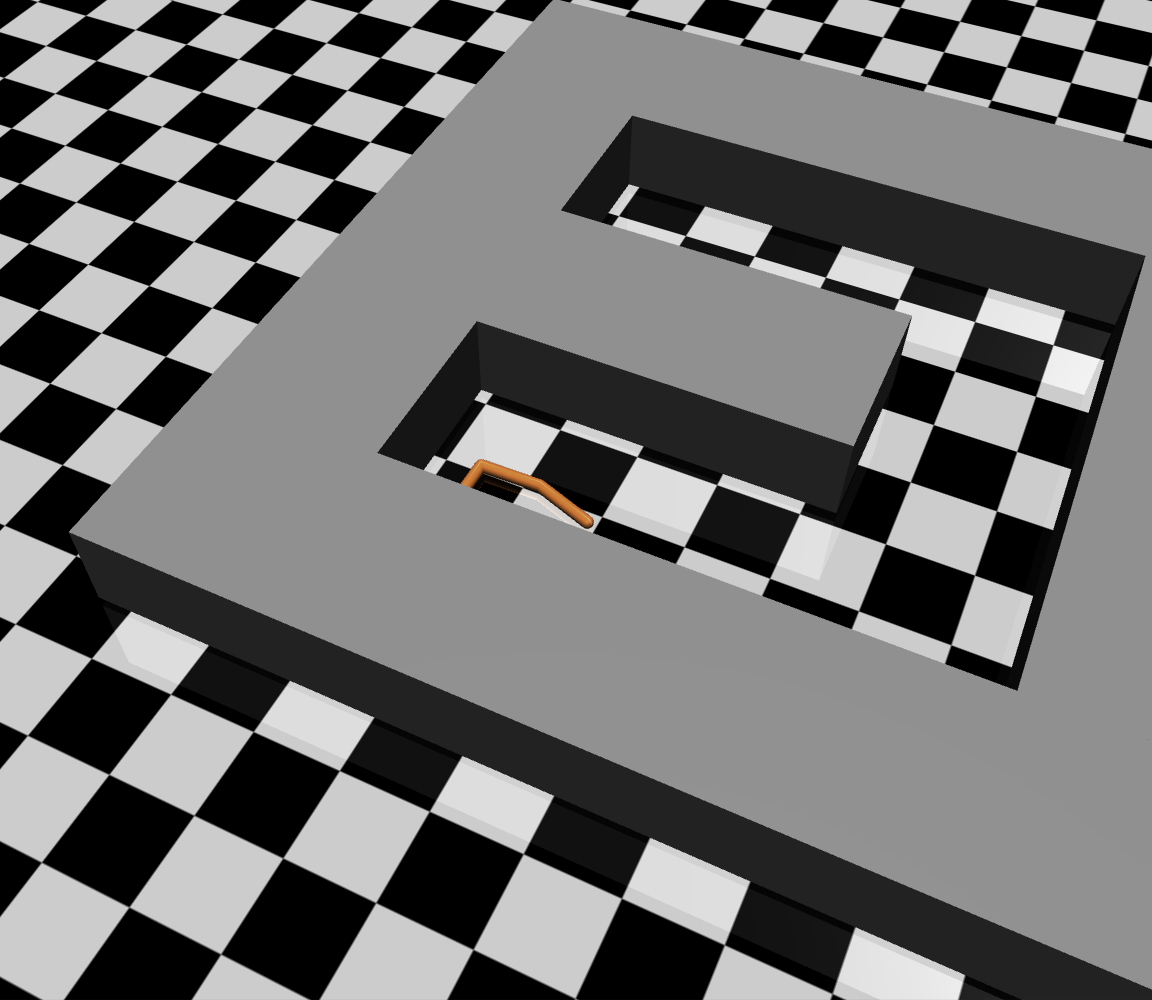
\includegraphics[width = 0.2\textwidth]{Figures/Maze0.png}
	}
	\subfigure[Bilinear integration]{
		\centering
		\label{fig:snn_architecture_bilinear}
		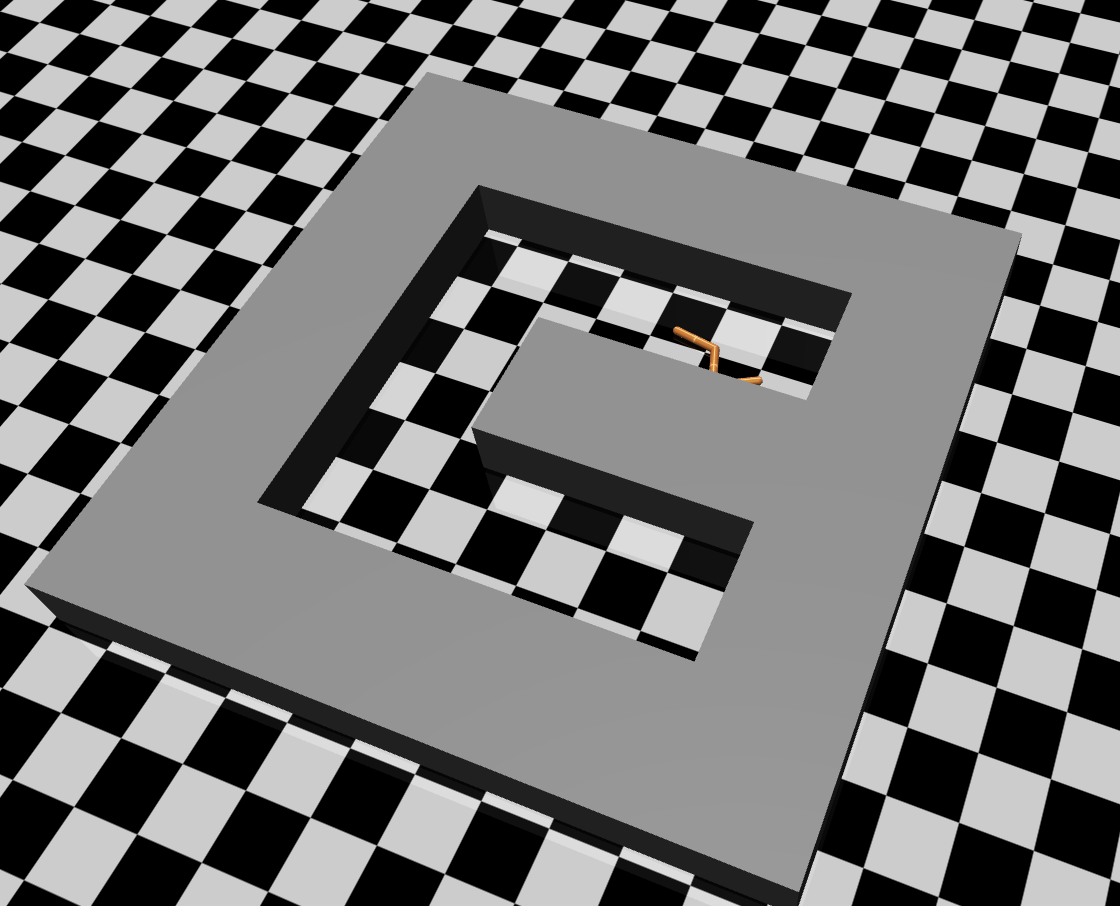
\includegraphics[width = 0.2\textwidth]{Figures/Maze10.png}
	}
	\caption{Different architectures for the integration of the latent variables in a FNN}
	\label{fig:snn_architecture}
\end{figure}

Note that the bilinear integration with one-hot vectors as proposed in Fig.\ \ref{fig:snn_bilinear} can be interpreted as changing the whole first layer of the FNN based on the latent code sampled. 

Even with the additional parameters needed to accomodate the enlarged input, SNNs are still much cheaper in parameters than training independent policies.\textit{ Re-trying only the first layer from the different policies trained sequentially will not grant a larger span of skills as most tries will fall in the same optima. <-- I have not checked that.. and even if I do, would I report that? Should this go in the experiments all together?}

\textit{This modification already yields a high span of skills so we haven't tried more/Other integrations could be explored}.

\subsection{Mutual Information bonus}
To further encourage the diversity of skills learned while training a SNN we introduce an information-theoretic based intrinsic reward. If many latents produce a motion of the robot towards the same region, it will be hard to infer what was the latent sampled at the beginning of the trajectory. Hence we can give a reward to every state based on how easily the latent is inferred. Formally we use the trajectories from the batch (and their latent) to obtain an empirical estimate of the posterior distribution $p(h|s)$ over latents given a state. Then the reward obtained in any sampled state $s_t$ is modified by $-\alpha_H H(p(h|s_t))$, where $\alpha_H$ is an hyperparameter that modulates the weight of this bonus. In parctice, this computation can be done very efficiently by gridding the space and counting the number of times each latent visited each grid. \textit{introduce the grid meshing hyperparameter here?}. Then the posterior $p(h_i|s_t)$ is simply taken as the ration of frequencies between the number of times states belonging to trajectories with latent $h_i$ visited the cell $n_h$ and total visitations of the cell $n_T$. Then the reward becomes $-\log(\frac{n_h}{n_T}$. \textit{Review this, specify better that the state is associated to the cell, and then put super-scripts to the $n$s}

\subsection{Hierarchical re-use of skills}
The MDPs that we want to tackle have a highly sparse reward structure and trying to learn a good policy from scratch in that environment can take very long or be not possible for standard methods. We propose to use the skills learned in the pre-training task in a hierarchical way to overcome this difficulty and learn faster. Instead of learning the low level skills again, we propose to learn only how to select skills sequentially. To do so we introduce a new "Pilot/Operator/high-level/manager" policy $\mathcal{M}_i$ for each new MDP $m_i$. This policy receives as input the full state $s_t\in \mathcal{S_i}$ and outputs a one-hot vector of dimension equal to the number of pre-trained skills. This vector is then used to select a skill to be active for the following $T_{agg}$ steps. During this time the actions takes are exclusively based on the robot observations $s^R_t\subset s_t$ and the active skill, and given that $\mathcal{A}_i = \mathcal{A}_{in}$ these actions can directly be applied to the current MDP $m_i$.


For the multi-policy architecture, each entry of the one-hot is used to multiply the output of each of the pre-trained policies. Summing this weighted/masked outputs effectively yields the action corresponding to the selected skill. For the SNN architecture, the one-hot vector is directly inputed in place of the latent. See details in Fig.\ \ref{fig:snn_architecture}

Our implementation parametrized the categorical distribution of the manager with a Neural Network with a soft-max at the output. The pre-trained networks remain fixed during learning in the new MDP $m_i$, therefore despite sampling a discrete variables we can still obtain the derivative of the policy with respect to all the trainable parameters with standard back-propagation and any policy gradient algorithm can be used to train the manager network. In fact, given now the discrete nature of the output of the trainable part, other methods like DQN or even value iteration could be used, opening a new realm of possibilities. We will still use TRPO just for simplicity/coherence/??. \textit{should this already be in experiments?}


\section{Experiments}
We have applied our framework to solving with a 3-link swimmer four mazes and a gathering task. Mazes 0 and 1 are depicted in Fig.\ \ref{fig:Maze0}-\ref{fig:Maze1}, where the robot is shown in its starting position and has to reach the other end of the U turn. Mazes 2 and 3 are different instantiations of the environment shown in Fig.\ \ref{fig:Maze2} where the goal has been placed in the North-East or in the South-West corner respectively. A reward of 1 is only granted when the robot reaches the goal position. In the gathering task, the robot gets a reward of 1 for collecting green balls and a reward of -1 for the red ones, all of which are positioned randomly at the start of each rollout. The sensor readings of Maze 0 and the latter task are fully described in the benchmark of continuous control problems \citep{yuan2015rllab}, where it was shown that no general purpose algorithm could solve them.

\begin{figure}[h!]
	\centering
	\subfigure[Maze 0]{
		\centering
		\label{fig:Maze0}
		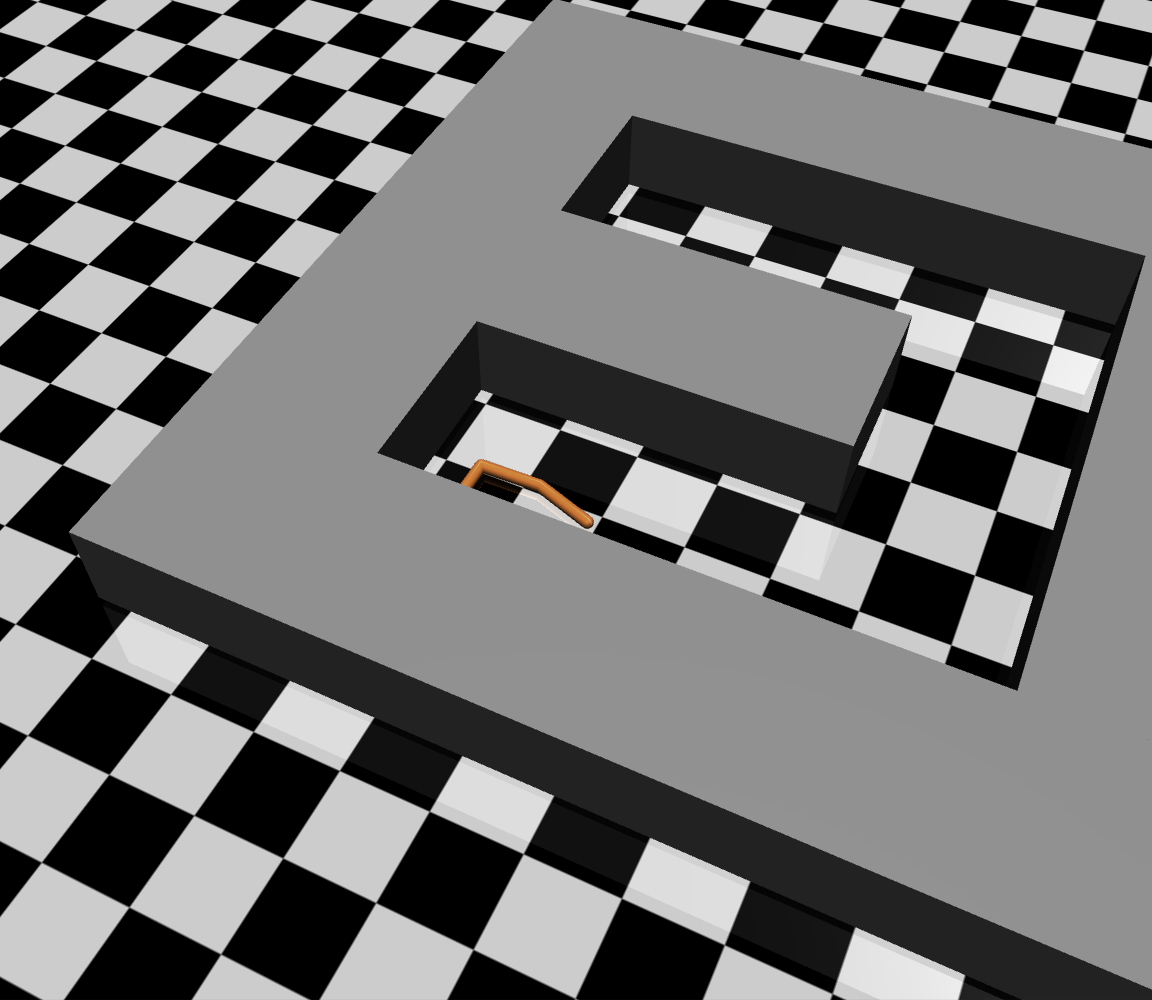
\includegraphics[width = 0.2\textwidth]{Figures/Maze0.png}
	}
	\subfigure[Maze 1]{
		\centering
		\label{fig:Maze1}
		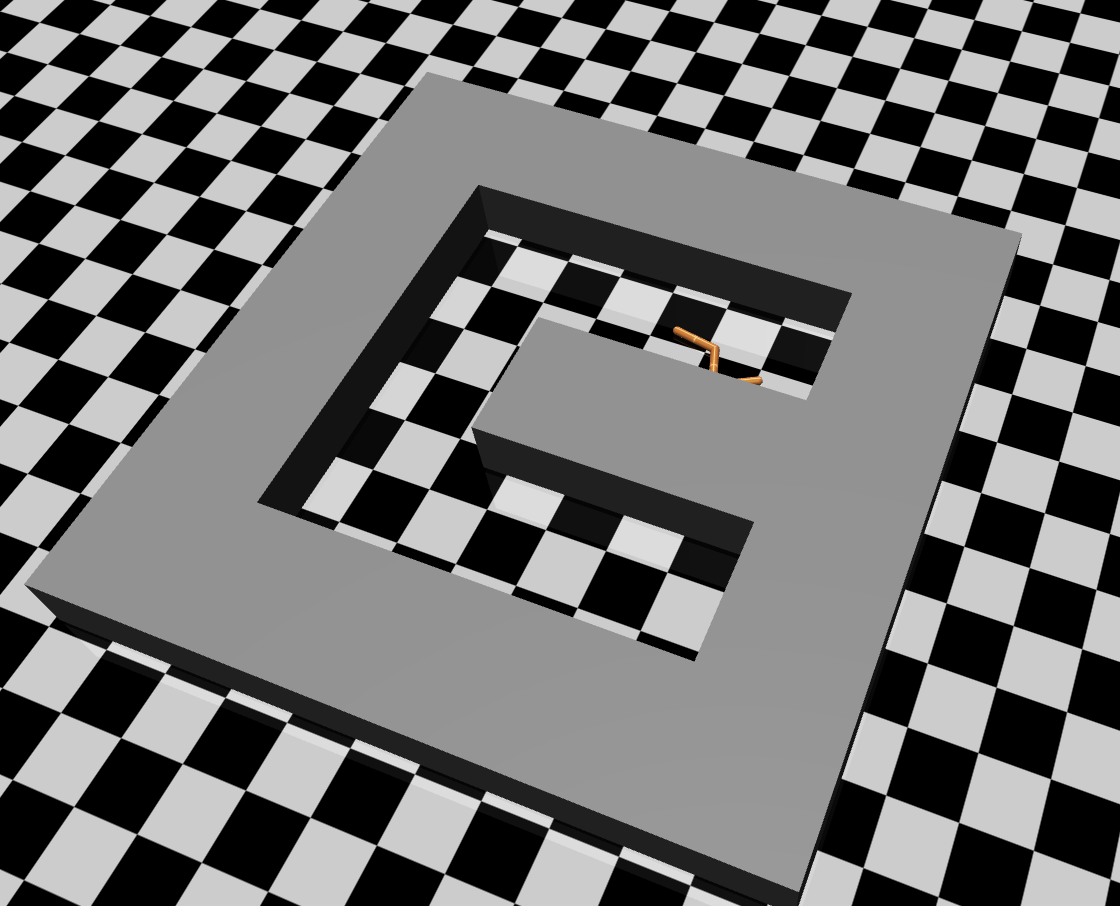
\includegraphics[width = 0.2\textwidth]{Figures/Maze10.png}
	}
	\subfigure[Maze 2 or 3]{
		\centering
		\label{fig:Maze2}
		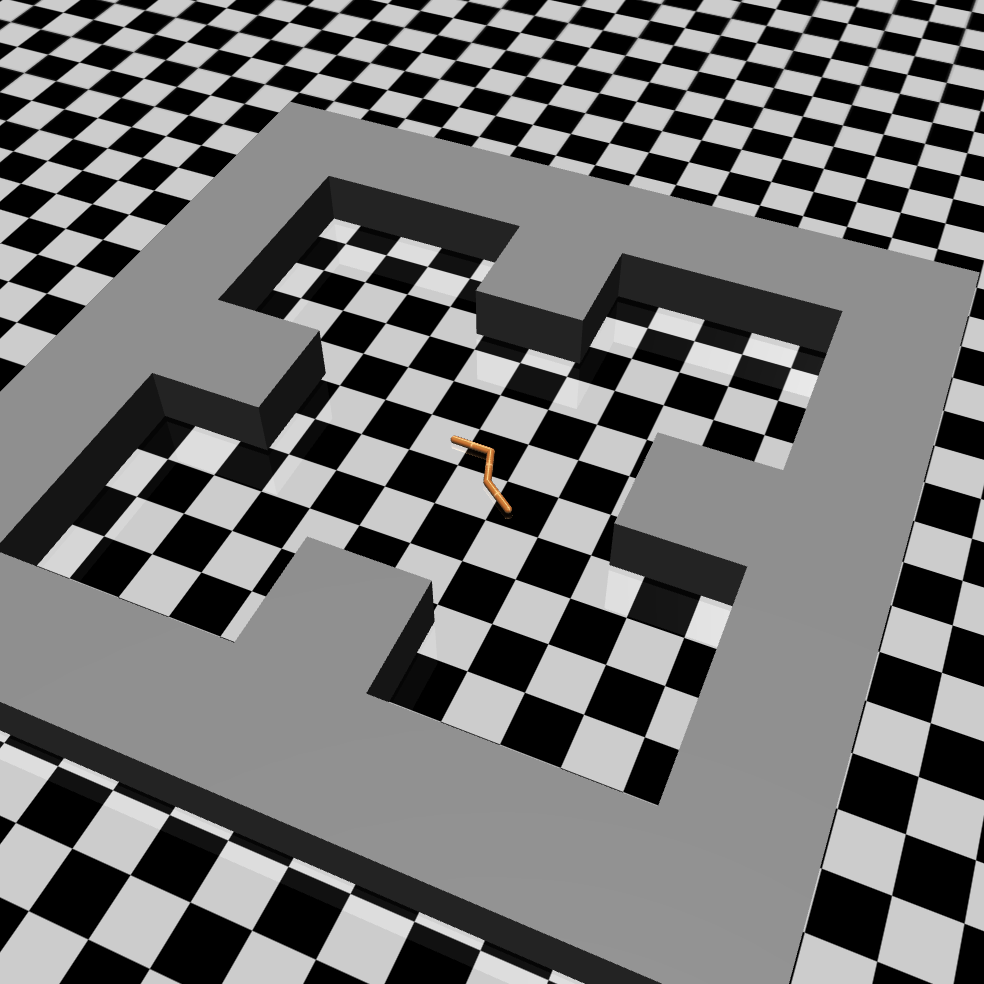
\includegraphics[width = 0.2\textwidth]{Figures/Maze4.png}
	}
	\subfigure[Food Gather]{
		\centering
		\label{fig:FoodGather}
		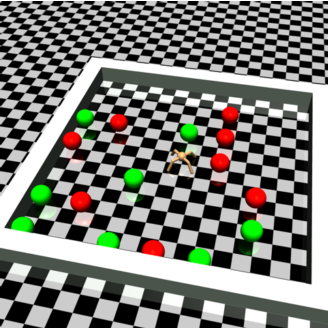
\includegraphics[width = 0.2\textwidth]{Figures/FoodGatherAnt.png}
	}
	\caption{Illustration of the sparse reward tasks}
	\label{fig:snn_multimodal_MI}
\end{figure}


The design parameters of our pre-train task and the next task are reported in Tab.\ \ref{tab:params} \textit{But in fact}

\begin{table}
\centering
\begin{tabular}[t]{ccc}
Parameter & multi-policy & SNN \\
\hline
number of skills & \multicolumn{2}{c}{6}\\
NN hidden units & \multicolumn{2}{c}{[32,32]}\\
Training algorithm & \multicolumn{2}{c}{TRPO}\\
Learning rate & \multicolumn{2}{c}{0.01}\\
\end{tabular}
\caption{Parameters of the model and algorithms}
\label{tab:params}
\end{table}

\section{Results}

First we evaluate the skill learning process, showing the relevance of the different pieces of our architecture and how they impact on the exploration achieved when using them in a hierarchical fashion. Then we report the results on the sparse environments described above.

\subsection{Skill learning}

Does pre-training with a general enough reward function yield a useful span of skills? To evaluate this we will use ``visitation plots'' showing the $(x,y)$ position of robot's Center of Mass (CoM) during 100 rollouts of 500 steps each. In Fig.\ \ref{fig:visit_trpo6} we show the visitation plot of 6 different policies, each trained from scratch in our pre-training environment. This yields 6 different ways of ``solving'' it. We can evaluate the combined span of skills with a visitation plot of the hierarchical multi-policy based on them, performing 100 rollouts of 1 aggregated step each, as seen in Fig.\ \ref{fig:visit_trpo6_likeSNN}. \textit{should I just say there that I plot them one on top of the other?} Given the morphology of the swimmer, it has an natural preference for forward and backward motion so when no extra incentive is added the visitation concentrates heavily on the direction it is initialized with.

Is it possible to obtain all this skills without having to train the policies independently? Fig.\ \ref{fig:visit_snn6_bilinear} shows the visitation plot of different SNN with bilinear integration and we see how each one of them has several "skills". Note how each latent generates a clearly interpretable behavior, despite not having any incentive to do so than the structure itself. These skills may overlap more or less but we have observed that 80\% of the trained SNN acquire at least forward and backward motion associated to different latents. On top of that, more turning skills than in Fig.\ \ref{fig:visit_trpo6_likeSNN} are observed, but without much consistency.

Can we increase the consistency and spread of skills obtained when training every SNN? Introducing the Mutual Information bonus derived above, both are achieved as can be observed in Fig.\ \ref{fig:visit_snn6_HB} showing the visitation plots obtained with different values of the bonus coeficient $\alpha_H$. Using only the Mutual Information bonus but not the bilinear integration also yields non-overlapping trajectories but it less conistentely yields at forward and backward motion as observed in Fig.\ \ref{fig:visit_snn6_noBil_HB}. Without bilinear integration the latents can't have a high level impact in the SNN and they are restricted to slighter variations of a certain motion.

\textit{Finally, is there any other reward than the CoM speed that would encourage the same span of skills? First, plots without that: only MI doesn't go far at all.}

\begin{figure}[h]
	\centering
	\subfigure[TRPO on regular NN]{
		\centering
		\label{fig:visit_trpo6}
	    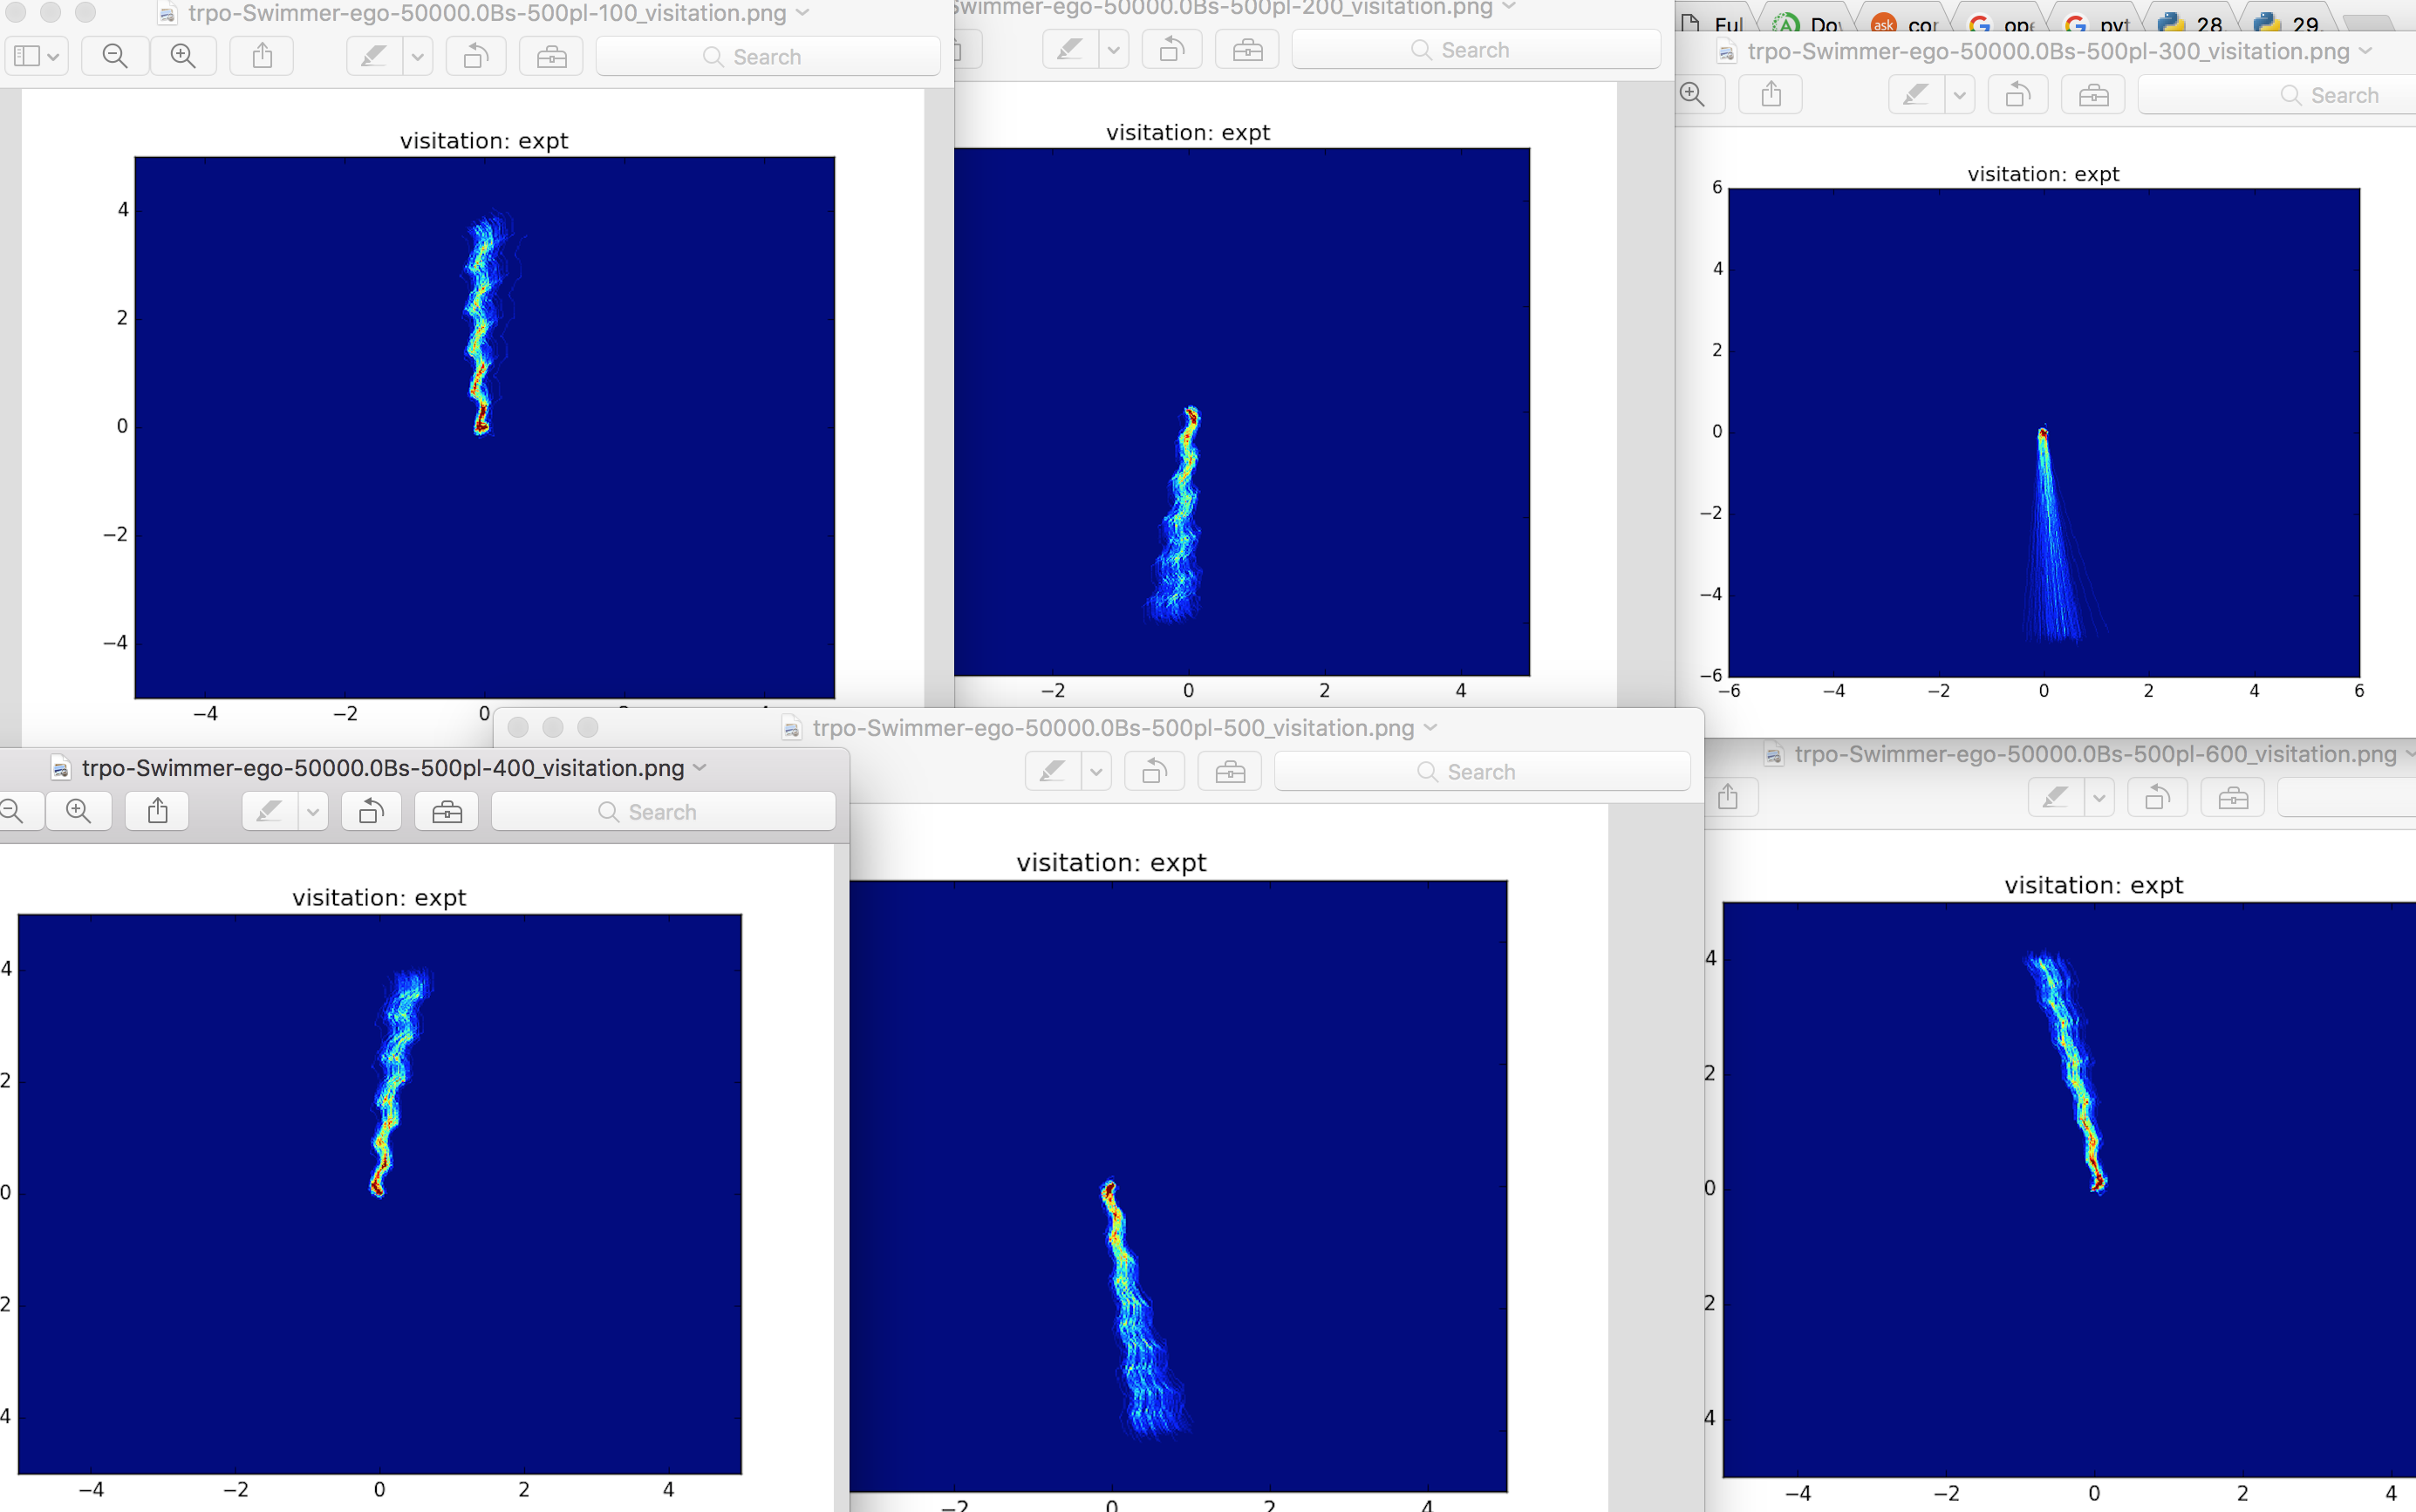
\includegraphics[width=0.4\textwidth]{Figures/visit_trpo6.png}
	}
	\subfigure[TRPO on regular NN]{
		\centering
		\label{fig:visit_trpo6_likeSNN}
	    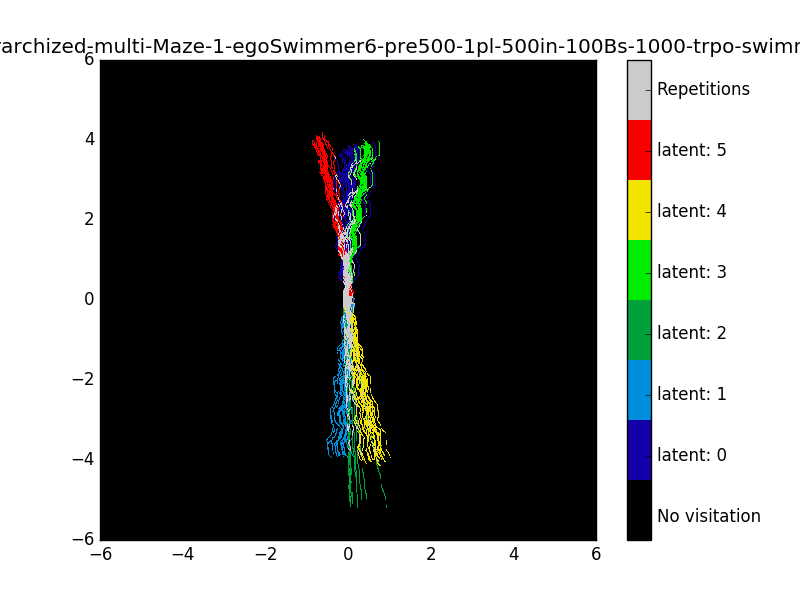
\includegraphics[width=0.4\textwidth]{Figures/likeSNN-hierarchized-multi-Maze-1-egoSwimmer6-pre500-1pl-500in-100Bs-1000-trpo-swimmer-ego-500_visitation.png}
	}
	\subfigure[SNN without bilinear integration]{
		\centering
		\label{fig:visit_snn6_noBilinear}
		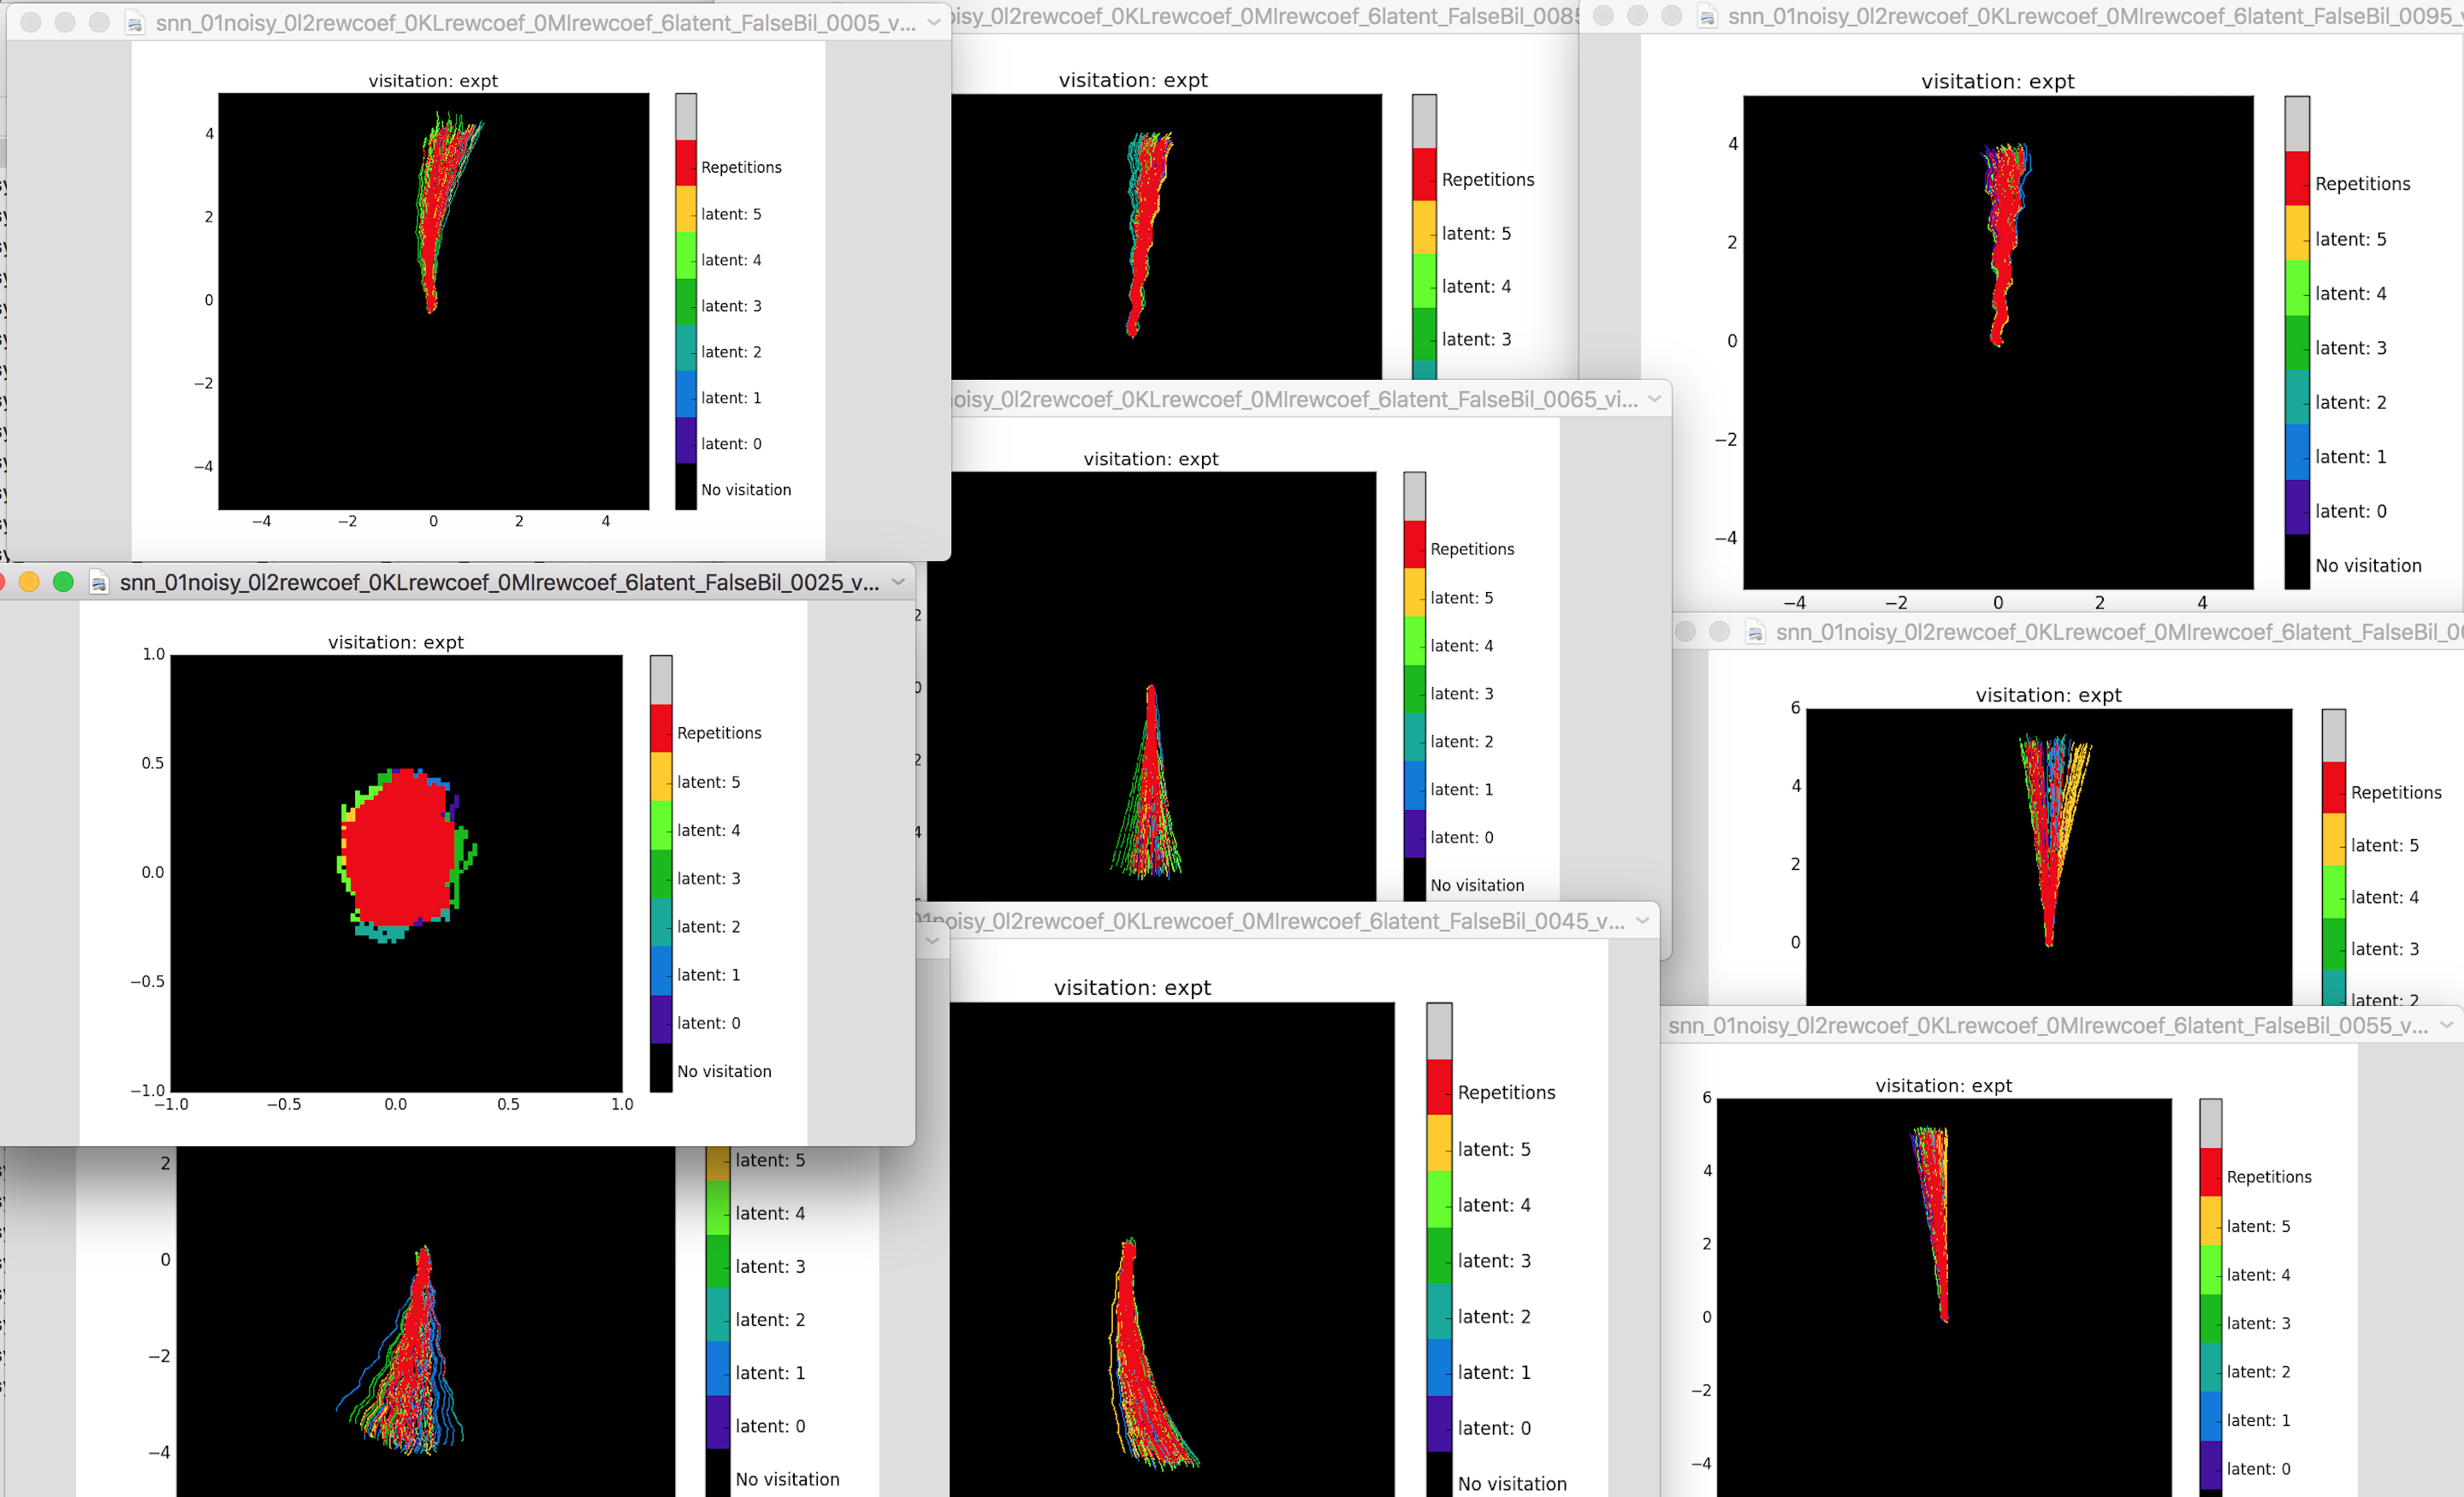
\includegraphics[width = 0.4\textwidth]{Figures/visit_snn_NoBil.png}
	}
	\subfigure[SNN with bilinear integration]{
		\centering
		\label{fig:visit_snn6_bilinear}
		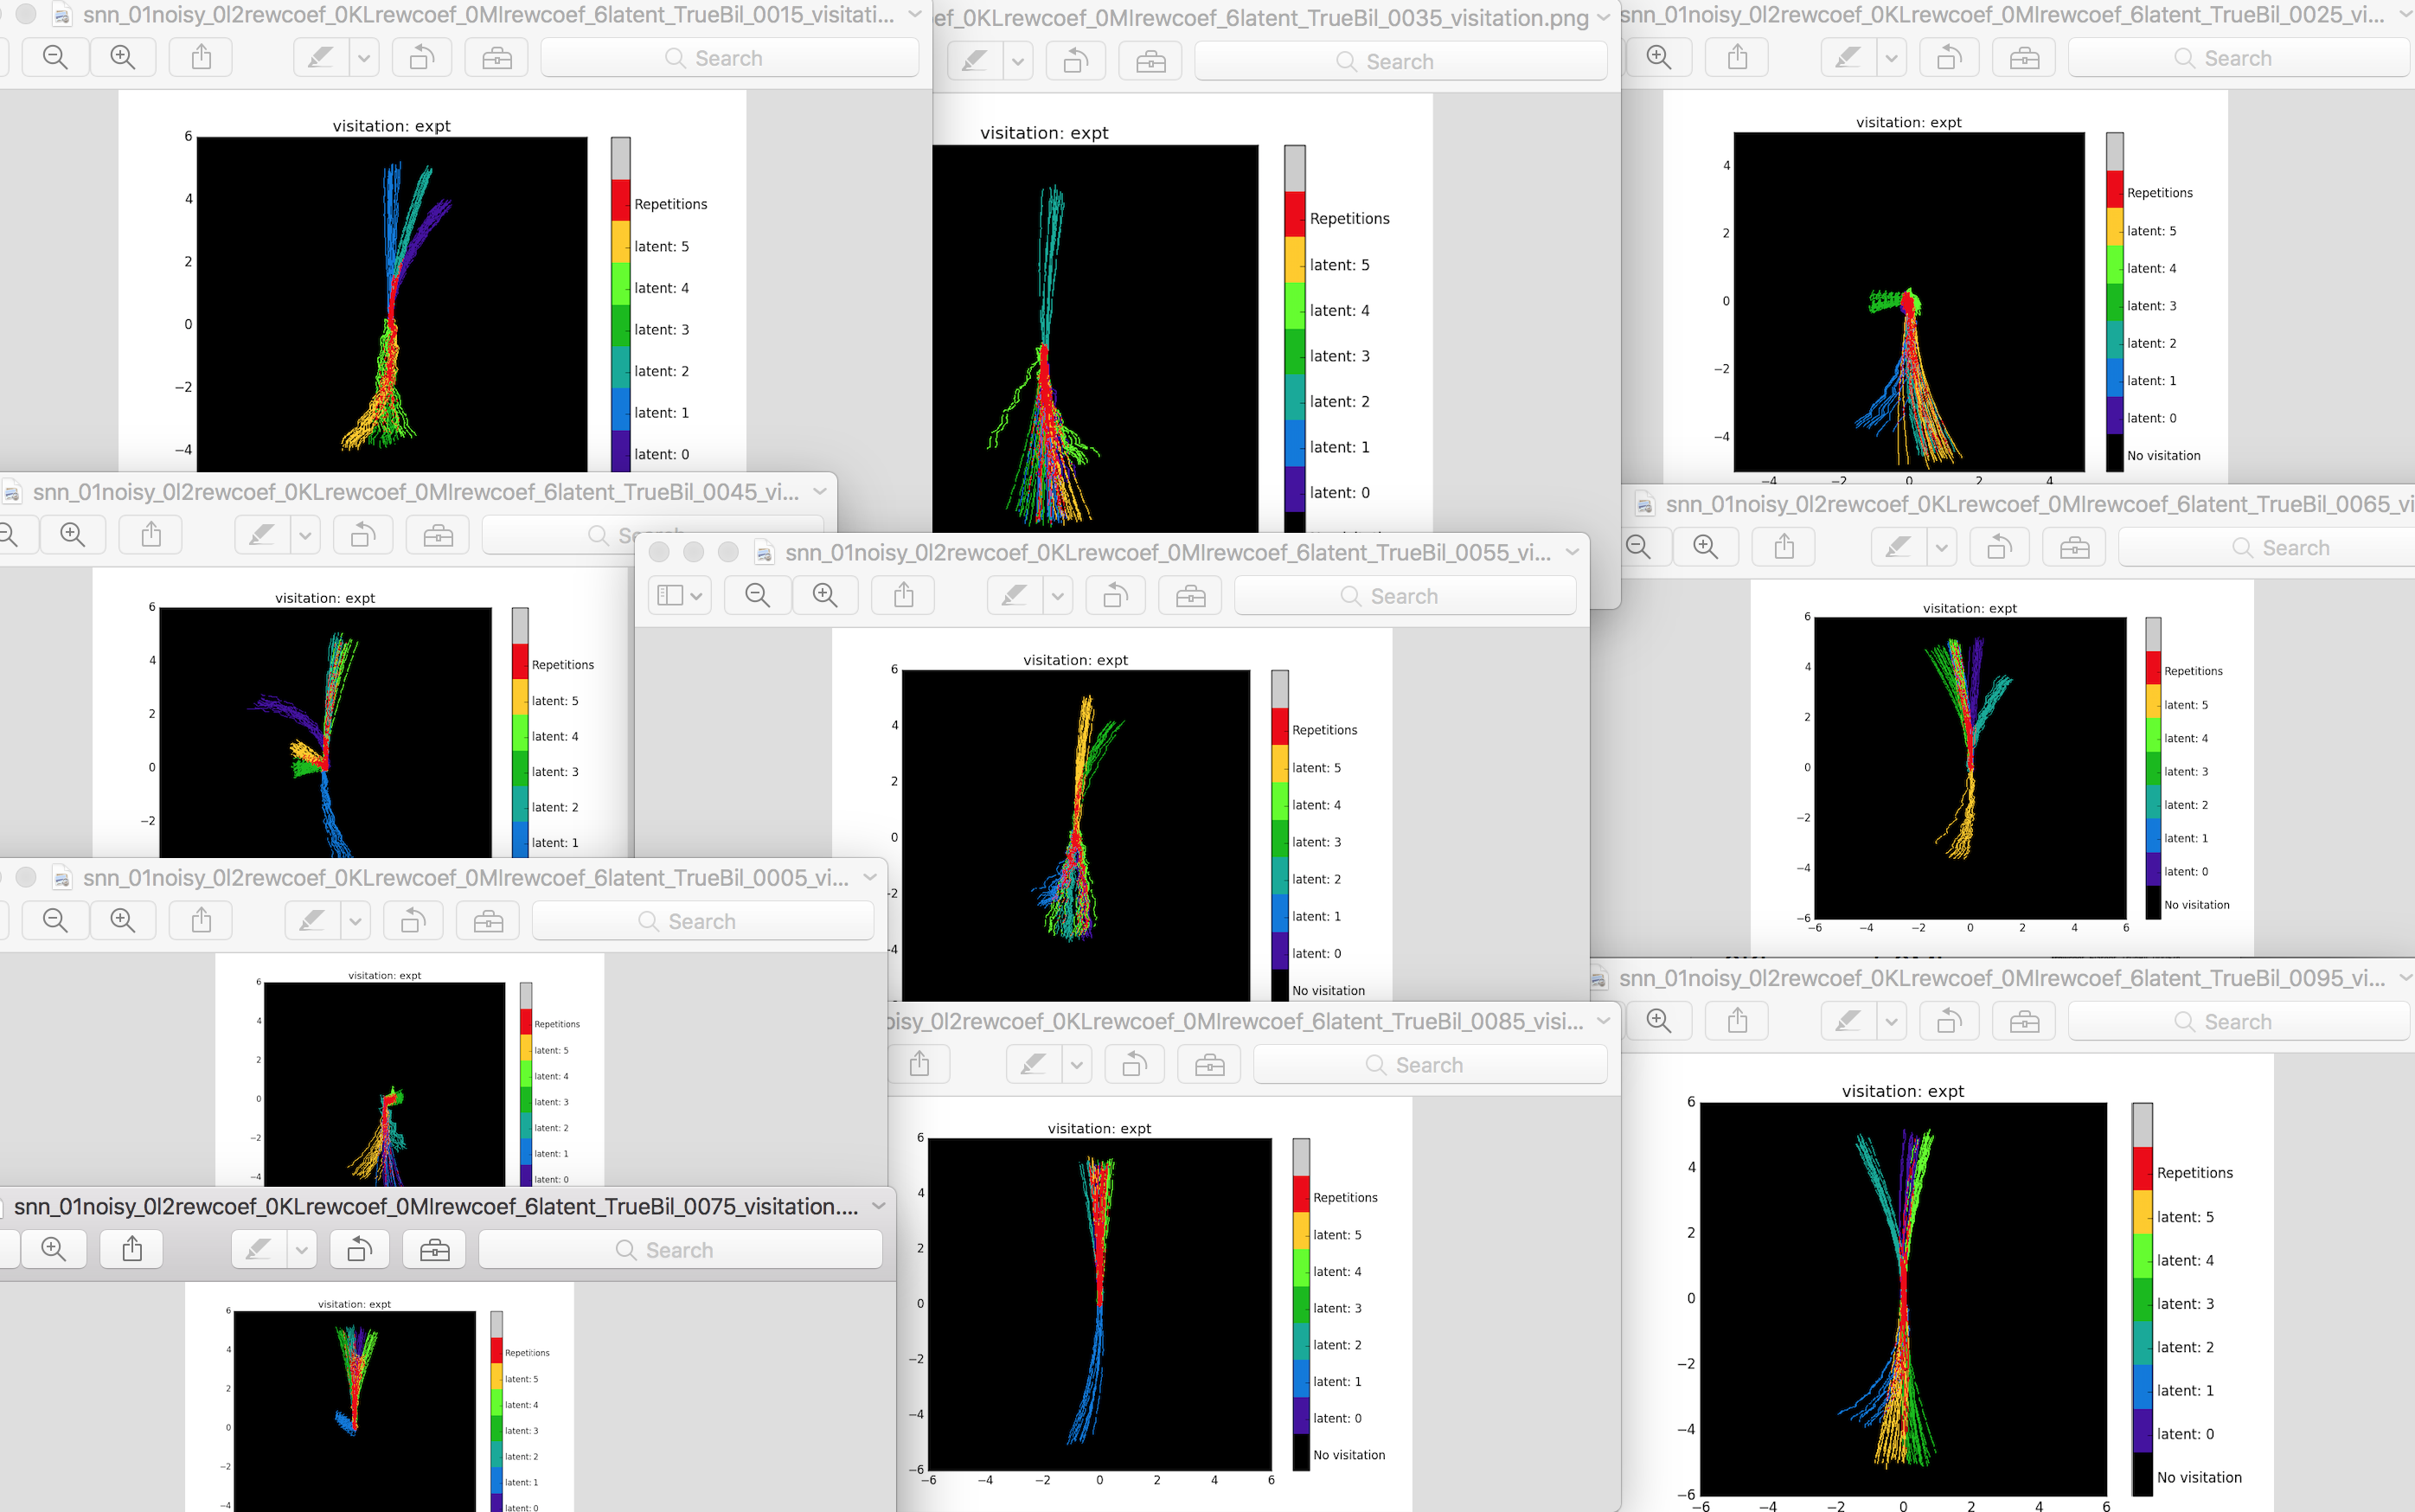
\includegraphics[width = 0.4\textwidth]{Figures/visit_snn6.png}
	}
	\subfigure[SNN with Hbonus integration VARYING!!]{
		\centering
		\label{fig:visit_snn6_HB}
		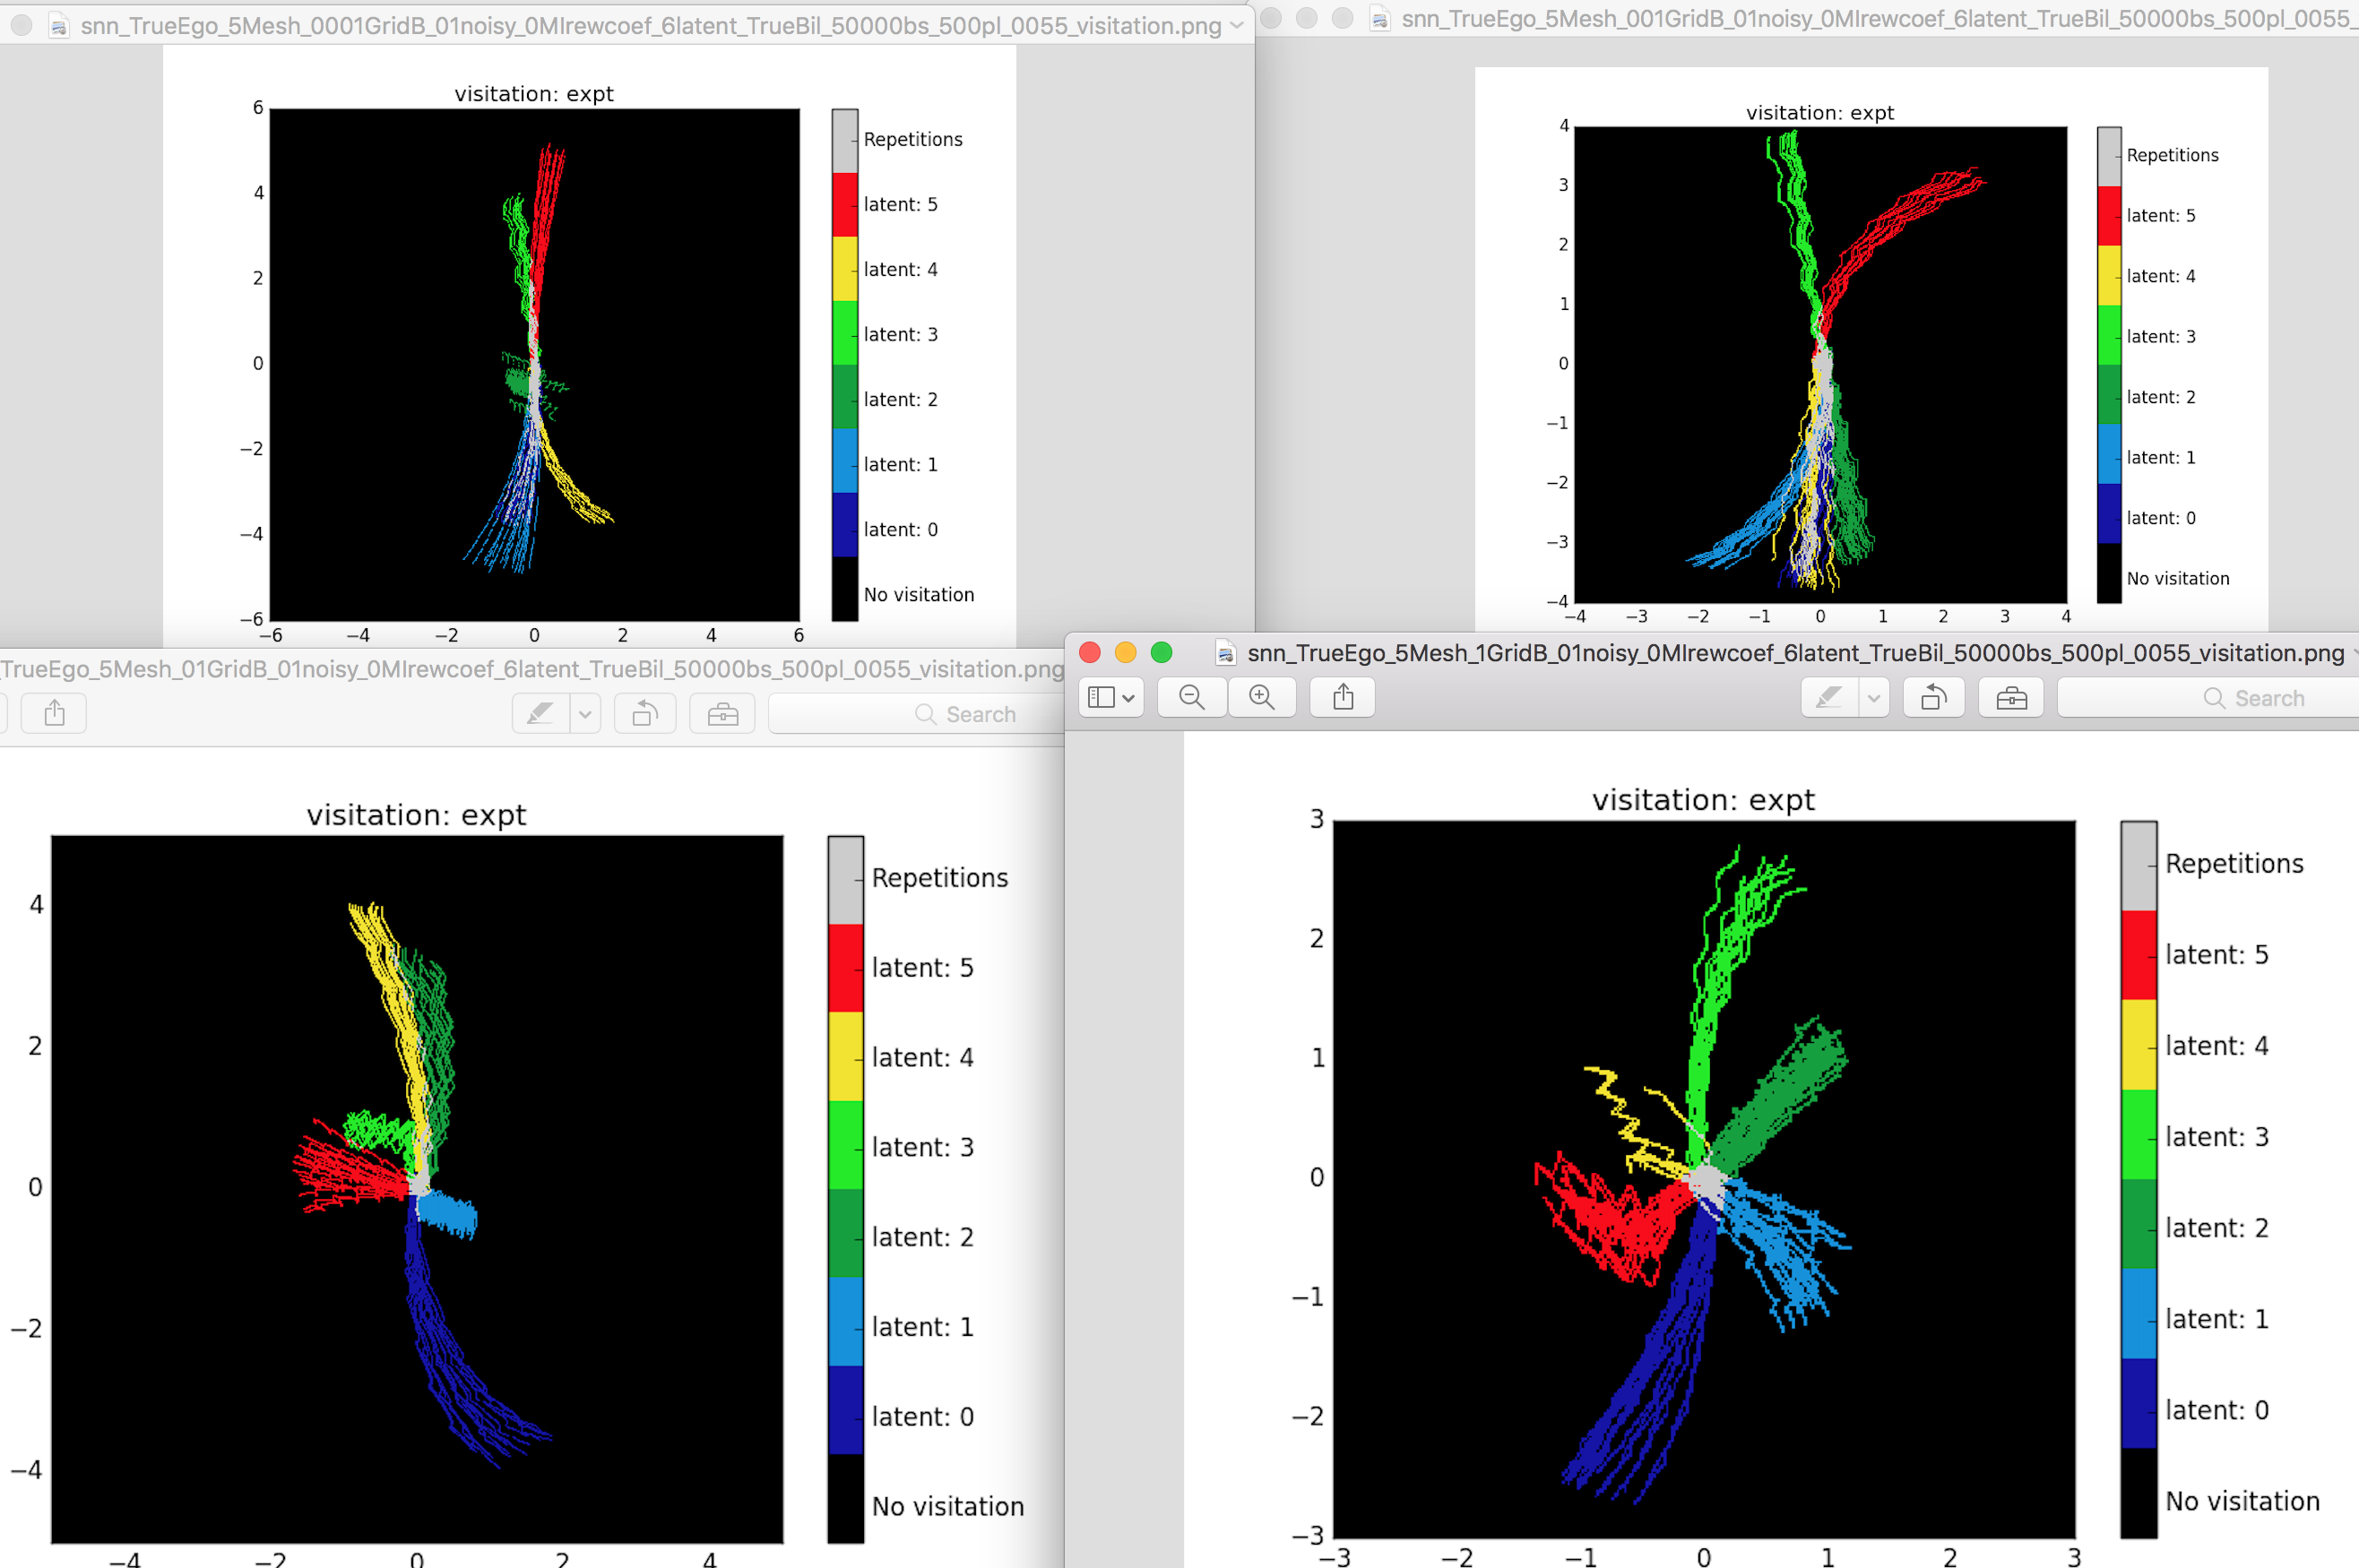
\includegraphics[width = 0.4\textwidth]{Figures/visit_snn_HB_varyCoef.png}
	}
	\subfigure[SNN with Hbonus integrationXXXXX]{
		\centering
		\label{fig:visit_snn6_noBil_HB}
		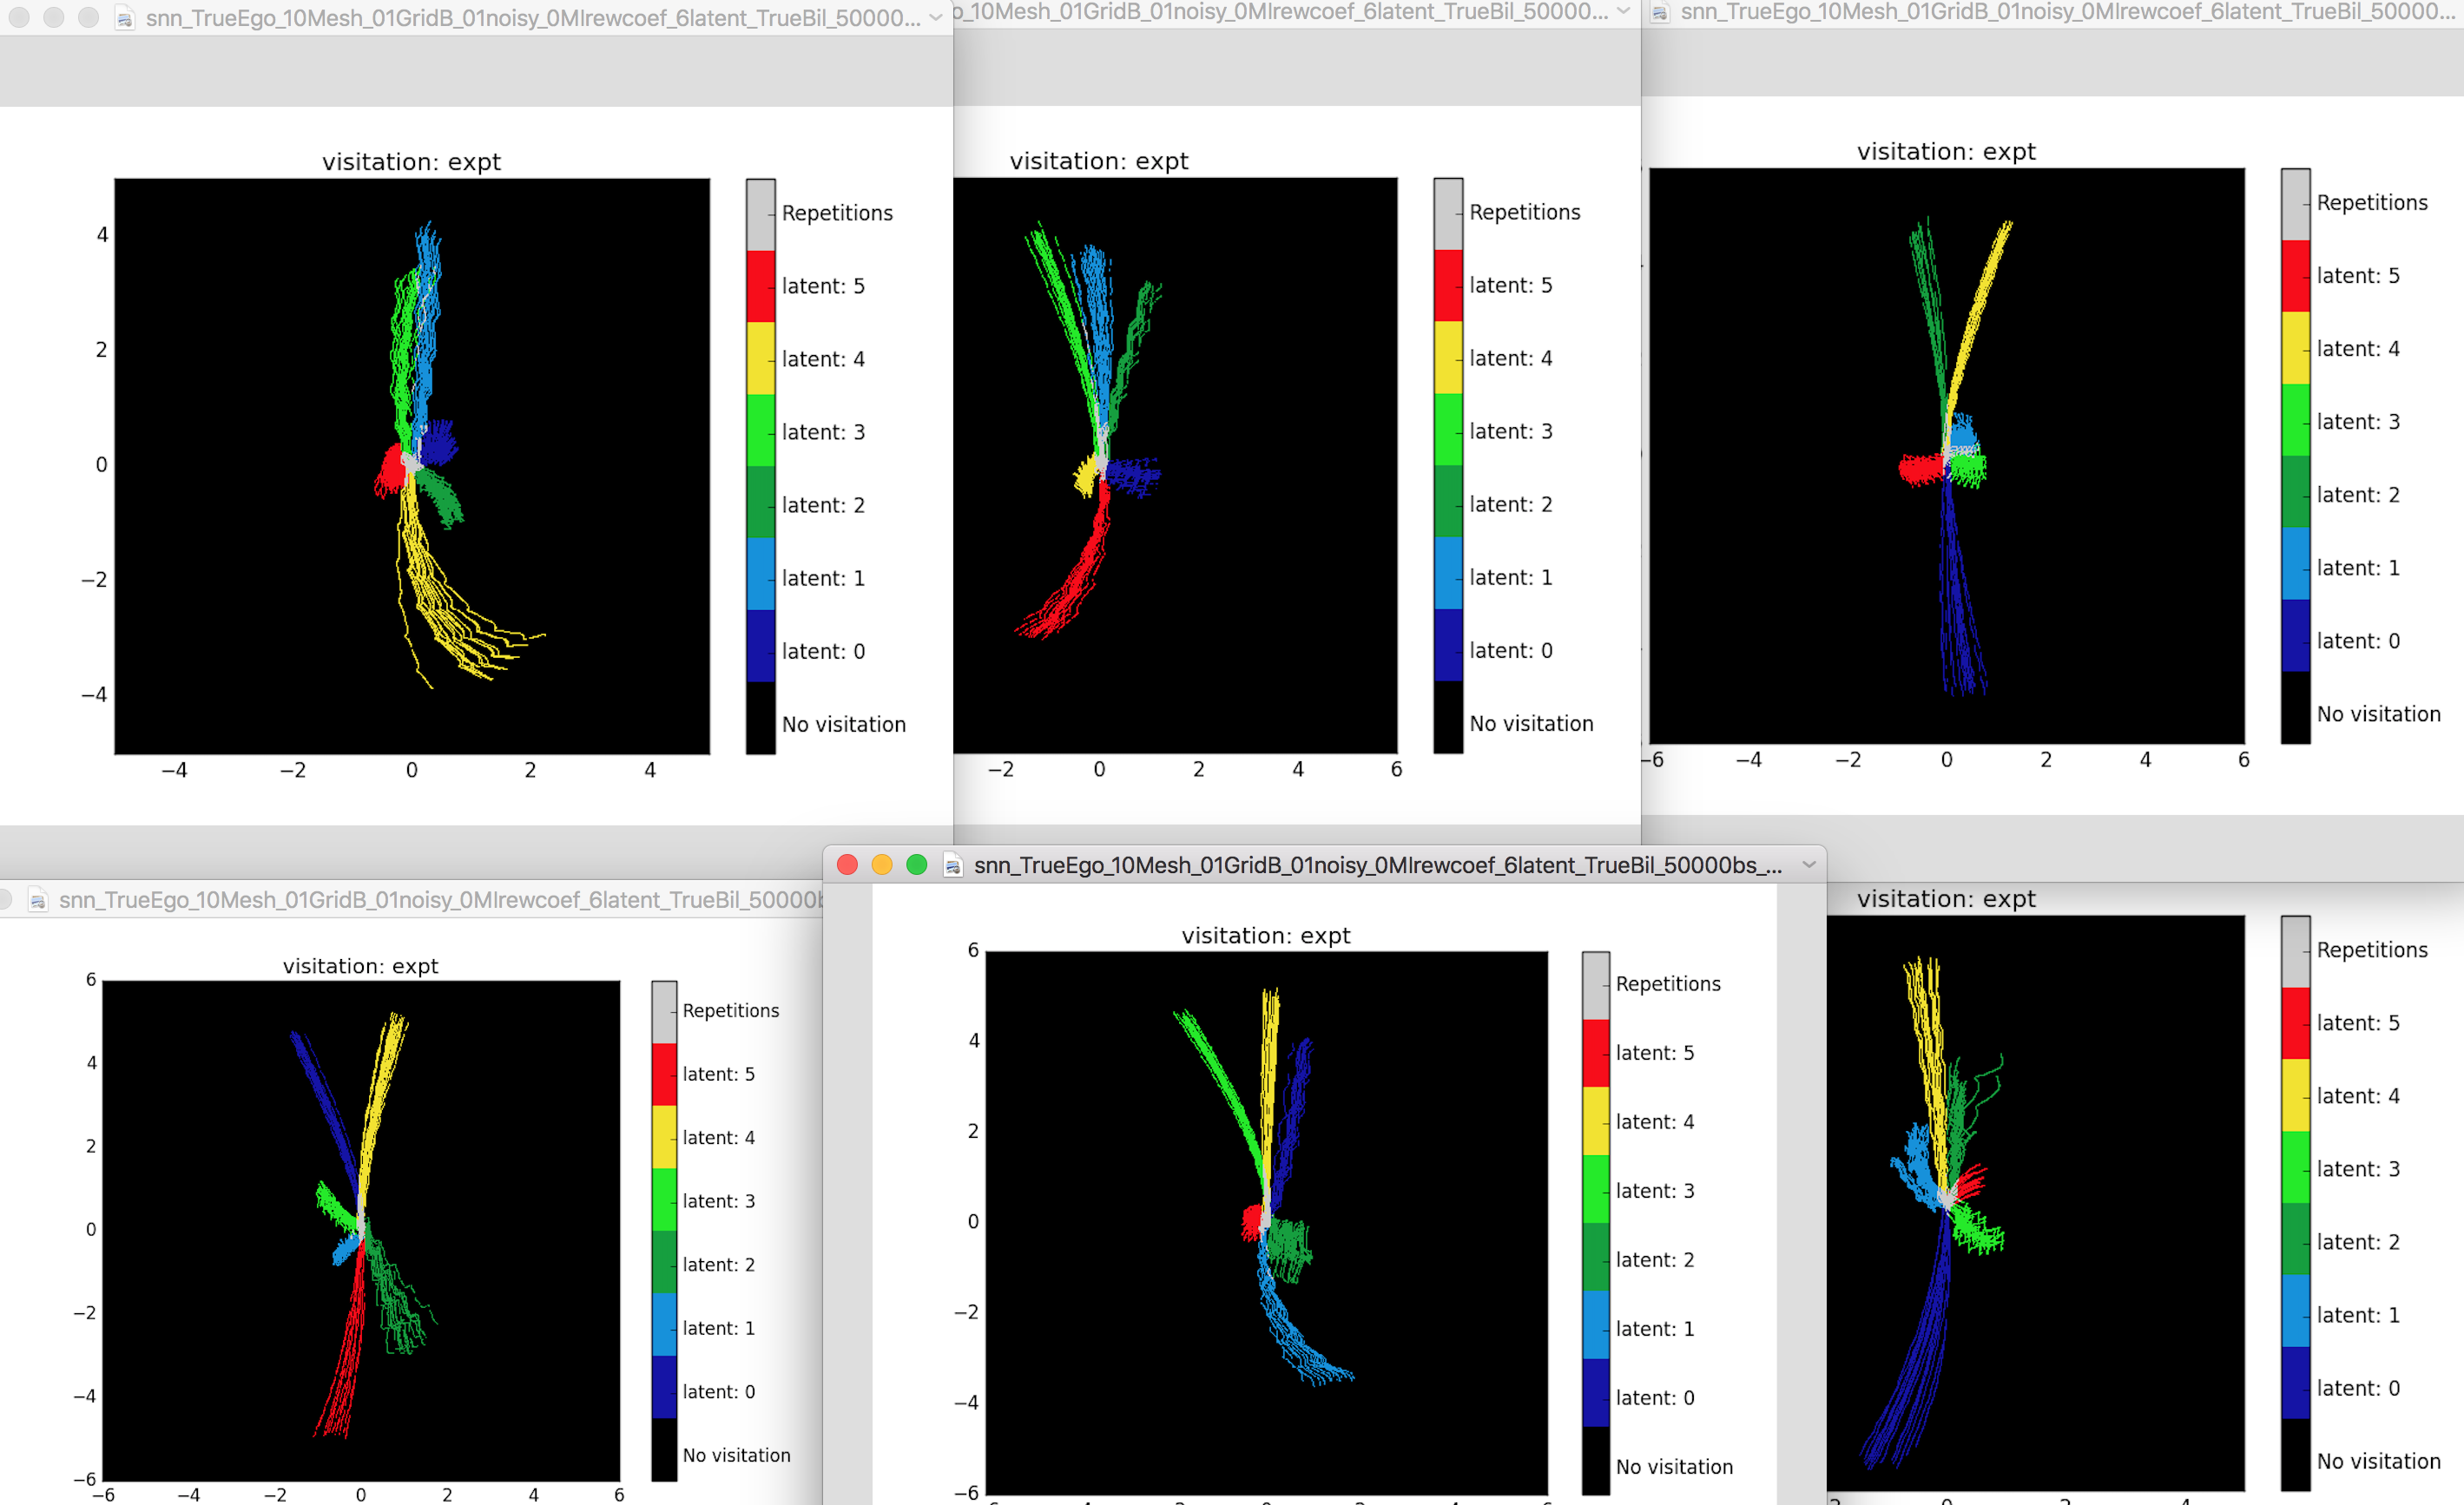
\includegraphics[width = 0.4\textwidth]{Figures/visit_snn_HB.png}
	}
	\caption{Span of skills learn by different methods and architectures}
	\label{fig:visit_methods}
\end{figure}


\subsection{Hierarchical use of skills}

Is it possible to leverage the pre-training experience to improve the exploration in future environments? The hierarchical architectures we have proposed have a very direct impact in the area covered by random exploration. We will examine these with visitation plots of 100 rollouts of length 10.000 for the different architectures. Fig.\ \ref{fig:visit-trpo1M} corresponds to Gaussian noise at the output with $\mu=0$ and $\Sigma=I$, as usually used in the first iteration of policy gradient methods (like our pre-training task). The swimmer robot has actions clipped to $[-1,1]$, so this noise is relatively very large \textit{and no other value consistently increases the total visitation}. In Fig.\ \ref{fig:visit-hier-multi-1M} we observe the drastic increase in exploration using the hierarchical approach with pre-trained policies. This plot shows a possible first iteration in the training of the manager network, hence being randomly initialize and picking policies almost uniformly, and committing to them for 500 steps. The same setup for SNNs with bilinear integration and $\alpha_H= 0$ and 0.1 can be seen in Figs.\ \ref{fig:visit-hier-snn-1M} and \ref{fig:visit-hier-snnHB-1M} respectively.

\begin{figure}[h!]
	\centering
	\subfigure[Gaussian noise exploration]{
		\centering
		\label{fig:visit-trpo-1M}
		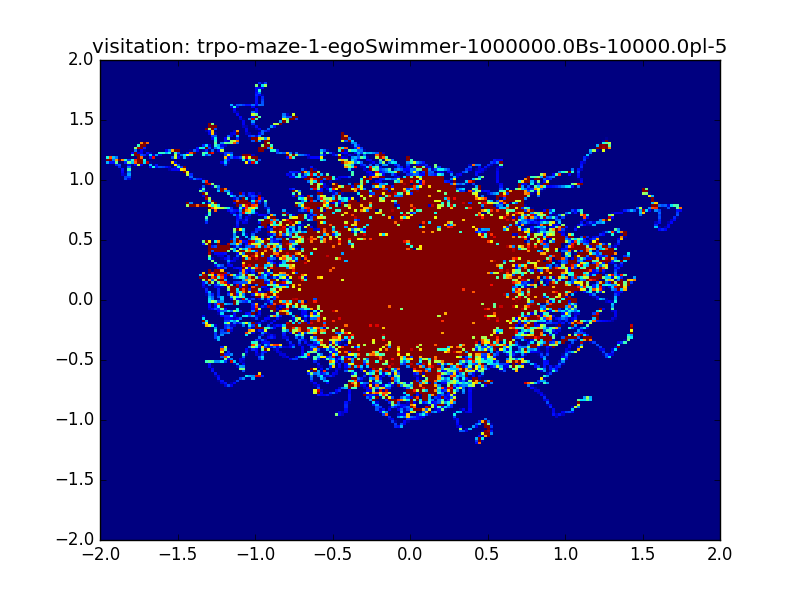
\includegraphics[width = 0.4\textwidth]{Figures/visit-trpo1M.png}
	}
	\subfigure[Exploration of the multi-policy hierarchical architecture]{
		\centering
		\label{fig:visit-multi-1M}
		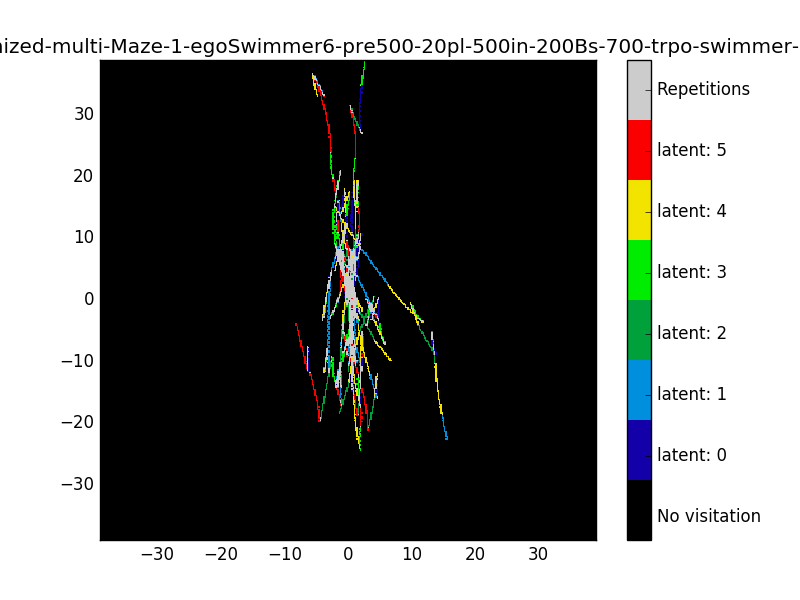
\includegraphics[width = 0.4\textwidth]{Figures/visit-multi-2.png}
	}
	\subfigure[visit-snn-1]{
		\centering
		\label{fig:visit-snnBil-1M}
		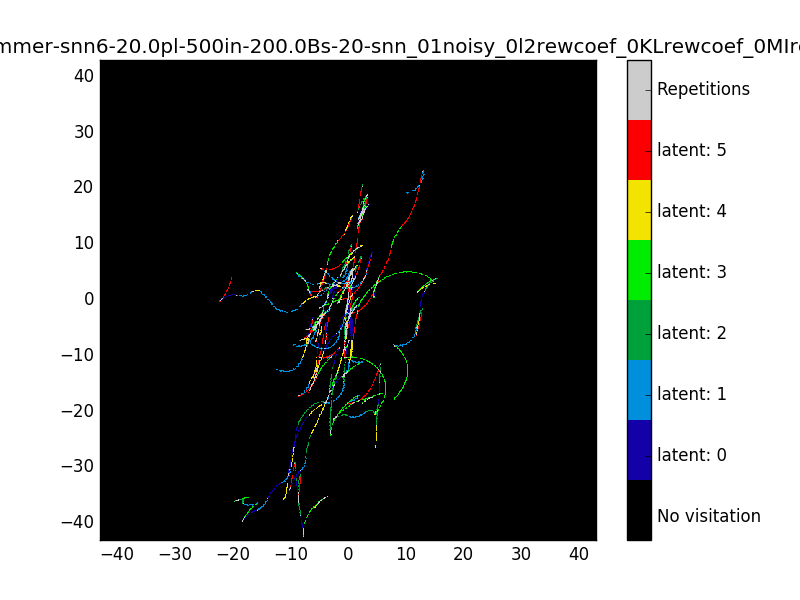
\includegraphics[width = 0.4\textwidth]{Figures/visit-snnBil-1M.png}
	}
	\subfigure[visit-snn-2]{
		\centering
		\label{fig:visit-hier-snnHB-1M}
		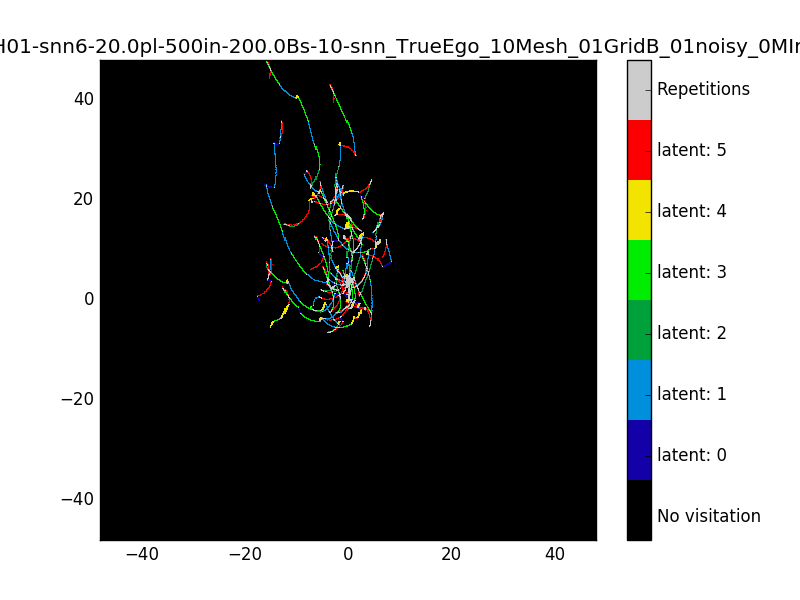
\includegraphics[width = 0.4\textwidth]{Figures/visit-snnHB-2.png}
	}
	\caption{Hierarchized exploration for multi-NN and SNN}
	\label{fig:hierarchized-exploration}
\end{figure}

\subsection{Maze 0 and 10}
The SNN are better!

\begin{figure}[h!]
	\centering
	\subfigure[Baseline: runnning iters w/ 1M bs]{
		\centering
		\label{fig:Maze4}
		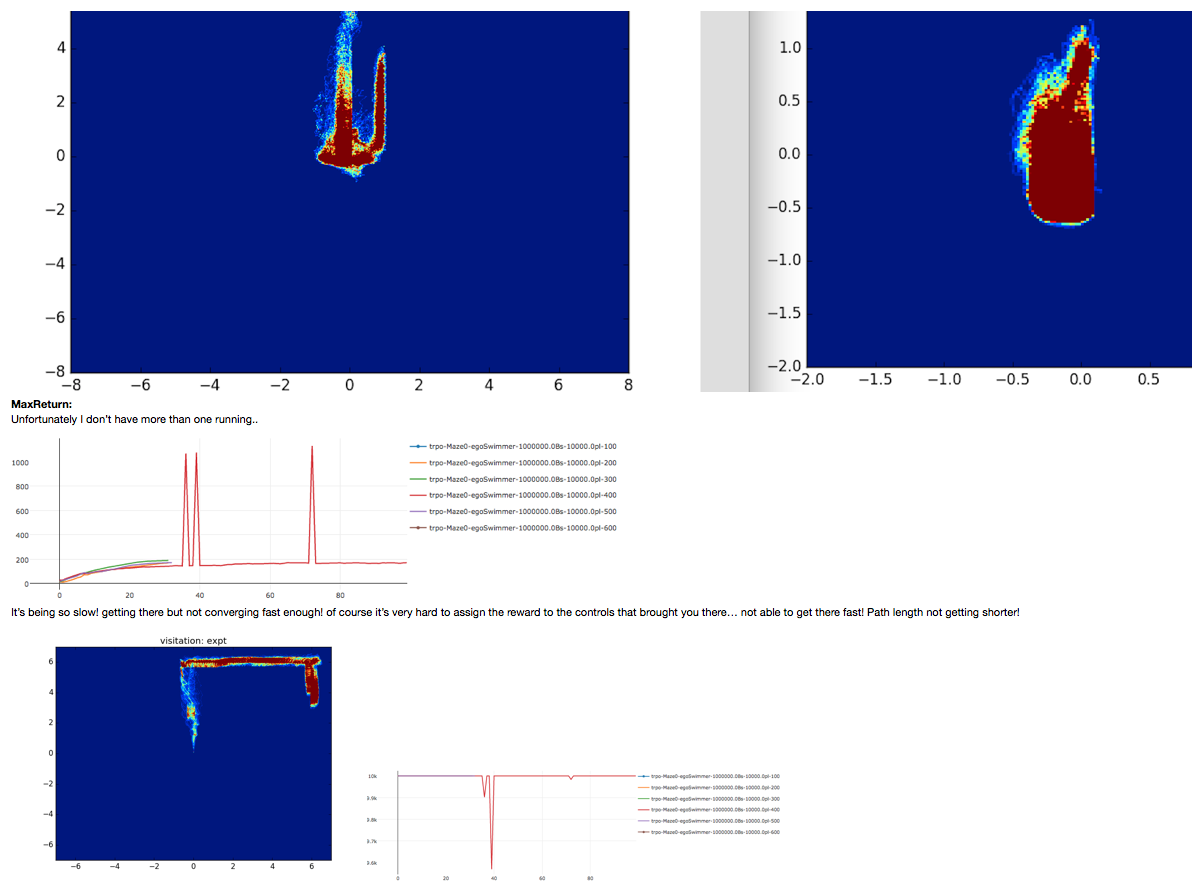
\includegraphics[width = 0.4\textwidth]{Figures/return_maze0_baseline.png}
	}
	\subfigure[visit-multi1]{
		\centering
		\label{fig:Maze0}
		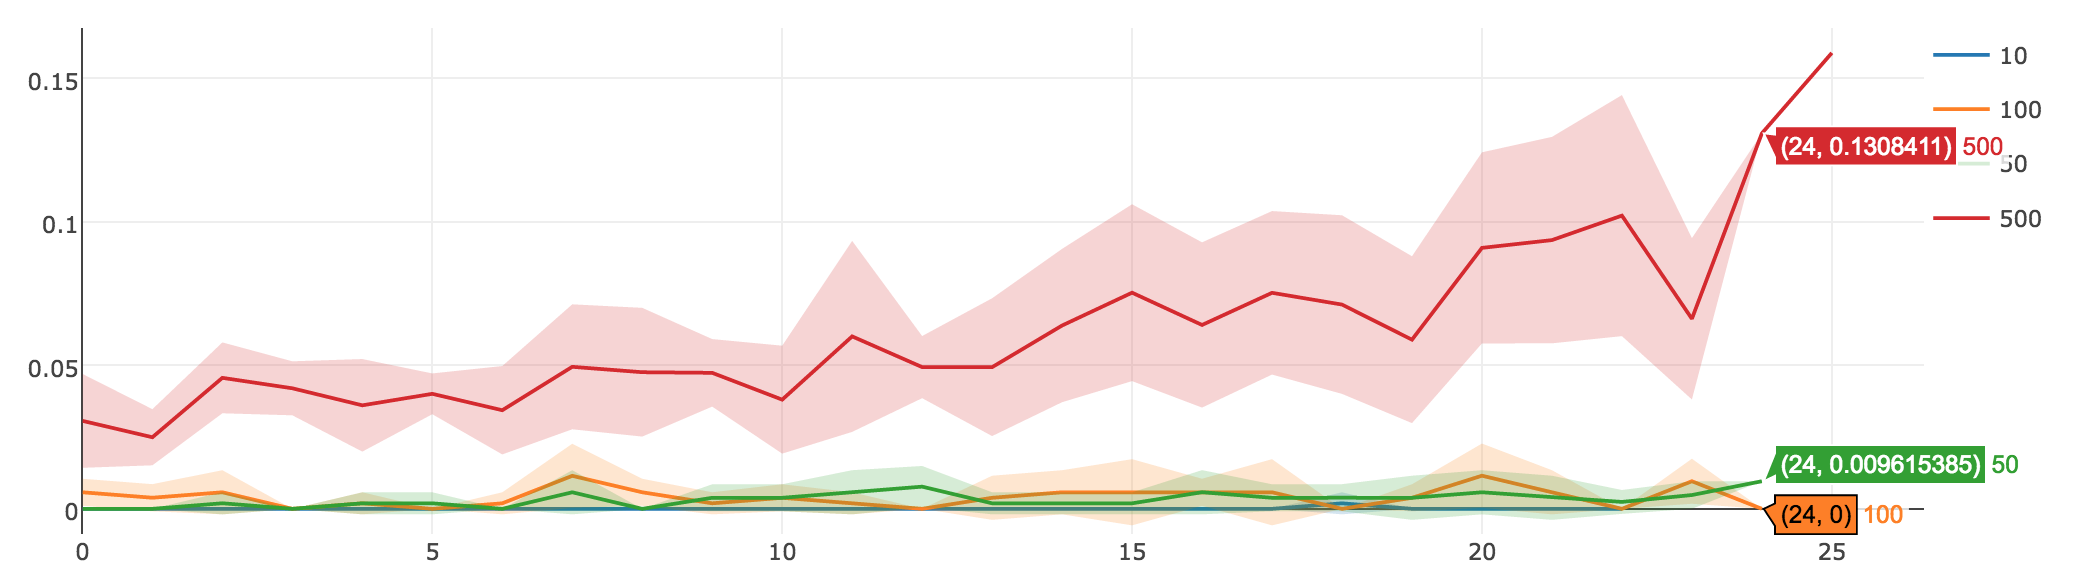
\includegraphics[width = 0.4\textwidth]{Figures/return_maze0_multi.png}
	}
	\subfigure[visit-multi2]{
		\centering
		\label{fig:FoodGather}
		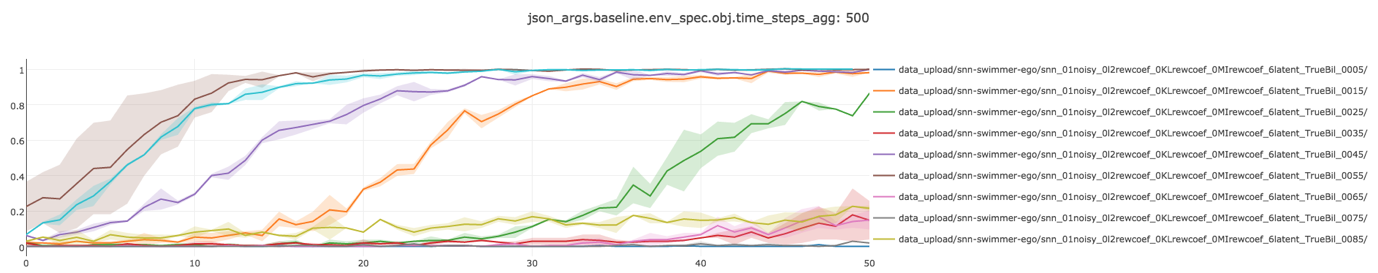
\includegraphics[width = 0.4\textwidth]{Figures/return_maze0_snn.png}
	}
	\subfigure[visit-snn-1]{
		\centering
		\label{fig:Maze10}
		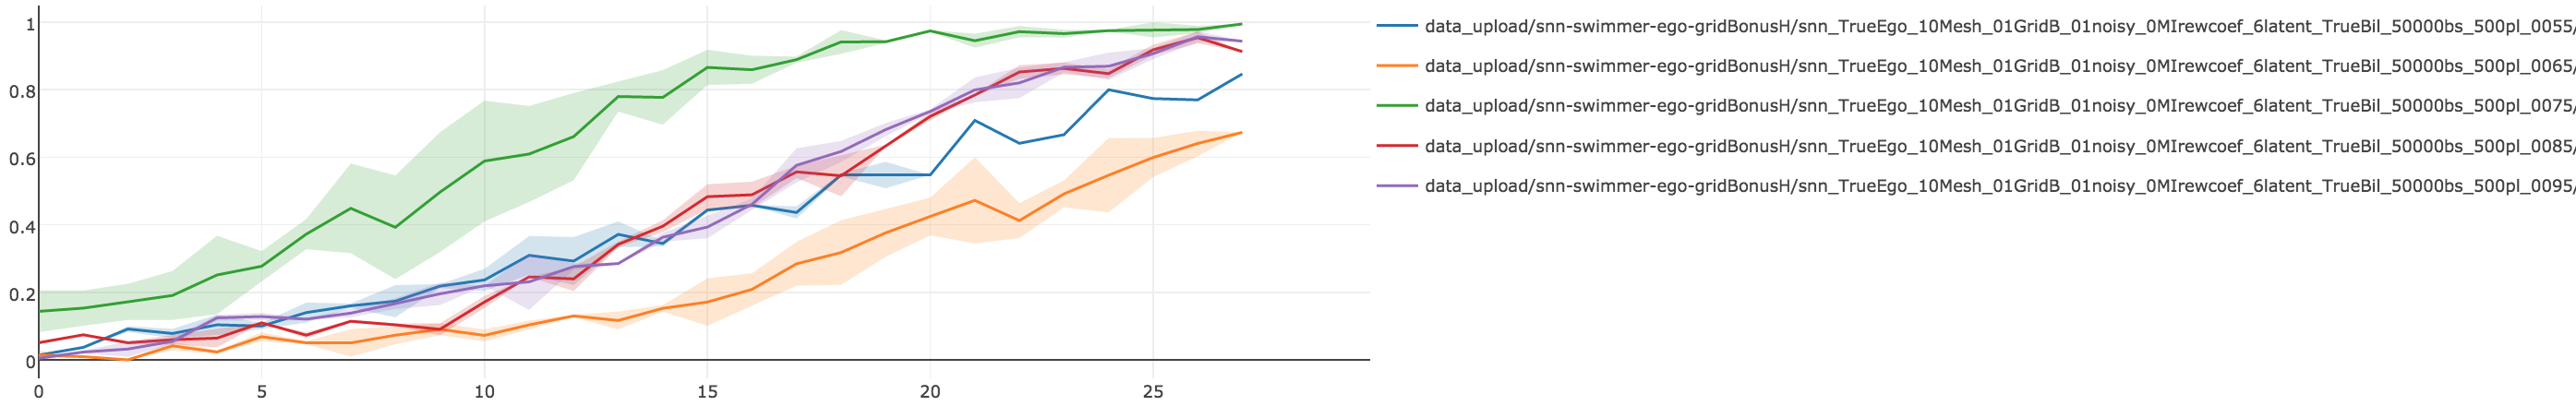
\includegraphics[width = 0.4\textwidth]{Figures/return_maze0_snnHB.png}
	}
	\caption{Maze0 - from RLLAB benchmark}
	\label{fig:hierarchized-exploration}
\end{figure}

\section{Conclusions}
We are the best

\subsubsection*{Acknowledgments}

\appendix
\section{Multimodal Policies in simple MDPs}
\textit{should we include here some of the work on 2D point-MDPs?}
\bibliography{ref}
\bibliographystyle{iclr2017_conference}

\end{document}
